% Options for packages loaded elsewhere
% Options for packages loaded elsewhere
\PassOptionsToPackage{unicode}{hyperref}
\PassOptionsToPackage{hyphens}{url}
\PassOptionsToPackage{dvipsnames,svgnames,x11names}{xcolor}
%
\documentclass[
  11pt,
  a4paper,
  DIV=11,
  numbers=noendperiod]{scrartcl}
\usepackage{xcolor}
\usepackage[lmargin=2cm,rmargin=2cm,tmargin=2cm,bmargin=2cm]{geometry}
\usepackage{amsmath,amssymb}
\setcounter{secnumdepth}{5}
\usepackage{iftex}
\ifPDFTeX
  \usepackage[T1]{fontenc}
  \usepackage[utf8]{inputenc}
  \usepackage{textcomp} % provide euro and other symbols
\else % if luatex or xetex
  \usepackage{unicode-math} % this also loads fontspec
  \defaultfontfeatures{Scale=MatchLowercase}
  \defaultfontfeatures[\rmfamily]{Ligatures=TeX,Scale=1}
\fi
\usepackage{lmodern}
\ifPDFTeX\else
  % xetex/luatex font selection
\fi
% Use upquote if available, for straight quotes in verbatim environments
\IfFileExists{upquote.sty}{\usepackage{upquote}}{}
\IfFileExists{microtype.sty}{% use microtype if available
  \usepackage[]{microtype}
  \UseMicrotypeSet[protrusion]{basicmath} % disable protrusion for tt fonts
}{}
\makeatletter
\@ifundefined{KOMAClassName}{% if non-KOMA class
  \IfFileExists{parskip.sty}{%
    \usepackage{parskip}
  }{% else
    \setlength{\parindent}{0pt}
    \setlength{\parskip}{6pt plus 2pt minus 1pt}}
}{% if KOMA class
  \KOMAoptions{parskip=half}}
\makeatother
% Make \paragraph and \subparagraph free-standing
\makeatletter
\ifx\paragraph\undefined\else
  \let\oldparagraph\paragraph
  \renewcommand{\paragraph}{
    \@ifstar
      \xxxParagraphStar
      \xxxParagraphNoStar
  }
  \newcommand{\xxxParagraphStar}[1]{\oldparagraph*{#1}\mbox{}}
  \newcommand{\xxxParagraphNoStar}[1]{\oldparagraph{#1}\mbox{}}
\fi
\ifx\subparagraph\undefined\else
  \let\oldsubparagraph\subparagraph
  \renewcommand{\subparagraph}{
    \@ifstar
      \xxxSubParagraphStar
      \xxxSubParagraphNoStar
  }
  \newcommand{\xxxSubParagraphStar}[1]{\oldsubparagraph*{#1}\mbox{}}
  \newcommand{\xxxSubParagraphNoStar}[1]{\oldsubparagraph{#1}\mbox{}}
\fi
\makeatother

\usepackage{color}
\usepackage{fancyvrb}
\newcommand{\VerbBar}{|}
\newcommand{\VERB}{\Verb[commandchars=\\\{\}]}
\DefineVerbatimEnvironment{Highlighting}{Verbatim}{commandchars=\\\{\}}
% Add ',fontsize=\small' for more characters per line
\usepackage{framed}
\definecolor{shadecolor}{RGB}{241,243,245}
\newenvironment{Shaded}{\begin{snugshade}}{\end{snugshade}}
\newcommand{\AlertTok}[1]{\textcolor[rgb]{0.68,0.00,0.00}{#1}}
\newcommand{\AnnotationTok}[1]{\textcolor[rgb]{0.37,0.37,0.37}{#1}}
\newcommand{\AttributeTok}[1]{\textcolor[rgb]{0.40,0.45,0.13}{#1}}
\newcommand{\BaseNTok}[1]{\textcolor[rgb]{0.68,0.00,0.00}{#1}}
\newcommand{\BuiltInTok}[1]{\textcolor[rgb]{0.00,0.23,0.31}{#1}}
\newcommand{\CharTok}[1]{\textcolor[rgb]{0.13,0.47,0.30}{#1}}
\newcommand{\CommentTok}[1]{\textcolor[rgb]{0.37,0.37,0.37}{#1}}
\newcommand{\CommentVarTok}[1]{\textcolor[rgb]{0.37,0.37,0.37}{\textit{#1}}}
\newcommand{\ConstantTok}[1]{\textcolor[rgb]{0.56,0.35,0.01}{#1}}
\newcommand{\ControlFlowTok}[1]{\textcolor[rgb]{0.00,0.23,0.31}{\textbf{#1}}}
\newcommand{\DataTypeTok}[1]{\textcolor[rgb]{0.68,0.00,0.00}{#1}}
\newcommand{\DecValTok}[1]{\textcolor[rgb]{0.68,0.00,0.00}{#1}}
\newcommand{\DocumentationTok}[1]{\textcolor[rgb]{0.37,0.37,0.37}{\textit{#1}}}
\newcommand{\ErrorTok}[1]{\textcolor[rgb]{0.68,0.00,0.00}{#1}}
\newcommand{\ExtensionTok}[1]{\textcolor[rgb]{0.00,0.23,0.31}{#1}}
\newcommand{\FloatTok}[1]{\textcolor[rgb]{0.68,0.00,0.00}{#1}}
\newcommand{\FunctionTok}[1]{\textcolor[rgb]{0.28,0.35,0.67}{#1}}
\newcommand{\ImportTok}[1]{\textcolor[rgb]{0.00,0.46,0.62}{#1}}
\newcommand{\InformationTok}[1]{\textcolor[rgb]{0.37,0.37,0.37}{#1}}
\newcommand{\KeywordTok}[1]{\textcolor[rgb]{0.00,0.23,0.31}{\textbf{#1}}}
\newcommand{\NormalTok}[1]{\textcolor[rgb]{0.00,0.23,0.31}{#1}}
\newcommand{\OperatorTok}[1]{\textcolor[rgb]{0.37,0.37,0.37}{#1}}
\newcommand{\OtherTok}[1]{\textcolor[rgb]{0.00,0.23,0.31}{#1}}
\newcommand{\PreprocessorTok}[1]{\textcolor[rgb]{0.68,0.00,0.00}{#1}}
\newcommand{\RegionMarkerTok}[1]{\textcolor[rgb]{0.00,0.23,0.31}{#1}}
\newcommand{\SpecialCharTok}[1]{\textcolor[rgb]{0.37,0.37,0.37}{#1}}
\newcommand{\SpecialStringTok}[1]{\textcolor[rgb]{0.13,0.47,0.30}{#1}}
\newcommand{\StringTok}[1]{\textcolor[rgb]{0.13,0.47,0.30}{#1}}
\newcommand{\VariableTok}[1]{\textcolor[rgb]{0.07,0.07,0.07}{#1}}
\newcommand{\VerbatimStringTok}[1]{\textcolor[rgb]{0.13,0.47,0.30}{#1}}
\newcommand{\WarningTok}[1]{\textcolor[rgb]{0.37,0.37,0.37}{\textit{#1}}}

\usepackage{longtable,booktabs,array}
\newcounter{none} % for unnumbered tables
\usepackage{calc} % for calculating minipage widths
% Correct order of tables after \paragraph or \subparagraph
\usepackage{etoolbox}
\makeatletter
\patchcmd\longtable{\par}{\if@noskipsec\mbox{}\fi\par}{}{}
\makeatother
% Allow footnotes in longtable head/foot
\IfFileExists{footnotehyper.sty}{\usepackage{footnotehyper}}{\usepackage{footnote}}
\makesavenoteenv{longtable}
\usepackage{graphicx}
\makeatletter
\newsavebox\pandoc@box
\newcommand*\pandocbounded[1]{% scales image to fit in text height/width
  \sbox\pandoc@box{#1}%
  \Gscale@div\@tempa{\textheight}{\dimexpr\ht\pandoc@box+\dp\pandoc@box\relax}%
  \Gscale@div\@tempb{\linewidth}{\wd\pandoc@box}%
  \ifdim\@tempb\p@<\@tempa\p@\let\@tempa\@tempb\fi% select the smaller of both
  \ifdim\@tempa\p@<\p@\scalebox{\@tempa}{\usebox\pandoc@box}%
  \else\usebox{\pandoc@box}%
  \fi%
}
% Set default figure placement to htbp
\def\fps@figure{htbp}
\makeatother





\setlength{\emergencystretch}{3em} % prevent overfull lines

\providecommand{\tightlist}{%
  \setlength{\itemsep}{0pt}\setlength{\parskip}{0pt}}



 


\usepackage{booktabs}
\usepackage{longtable}
\usepackage{array}
\usepackage{multirow}
\usepackage{wrapfig}
\usepackage{float}
\usepackage{colortbl}
\usepackage{pdflscape}
\usepackage{tabu}
\usepackage{threeparttable}
\usepackage{threeparttablex}
\usepackage[normalem]{ulem}
\usepackage{makecell}
\usepackage{xcolor}
\KOMAoption{captions}{tableheading}
\makeatletter
\@ifpackageloaded{caption}{}{\usepackage{caption}}
\AtBeginDocument{%
\ifdefined\contentsname
  \renewcommand*\contentsname{Table of contents}
\else
  \newcommand\contentsname{Table of contents}
\fi
\ifdefined\listfigurename
  \renewcommand*\listfigurename{List of Figures}
\else
  \newcommand\listfigurename{List of Figures}
\fi
\ifdefined\listtablename
  \renewcommand*\listtablename{List of Tables}
\else
  \newcommand\listtablename{List of Tables}
\fi
\ifdefined\figurename
  \renewcommand*\figurename{Figure}
\else
  \newcommand\figurename{Figure}
\fi
\ifdefined\tablename
  \renewcommand*\tablename{Table}
\else
  \newcommand\tablename{Table}
\fi
}
\@ifpackageloaded{float}{}{\usepackage{float}}
\floatstyle{ruled}
\@ifundefined{c@chapter}{\newfloat{codelisting}{h}{lop}}{\newfloat{codelisting}{h}{lop}[chapter]}
\floatname{codelisting}{Listing}
\newcommand*\listoflistings{\listof{codelisting}{List of Listings}}
\makeatother
\makeatletter
\makeatother
\makeatletter
\@ifpackageloaded{caption}{}{\usepackage{caption}}
\@ifpackageloaded{subcaption}{}{\usepackage{subcaption}}
\makeatother
\usepackage{bookmark}
\IfFileExists{xurl.sty}{\usepackage{xurl}}{} % add URL line breaks if available
\urlstyle{same}
\hypersetup{
  pdftitle={Why Have House Prices in Turkey Gone Up in the Last Ten Years?},
  pdfauthor={Ömer Furkan Demirci; Fatih Alper Vural},
  colorlinks=true,
  linkcolor={blue},
  filecolor={Maroon},
  citecolor={Blue},
  urlcolor={Blue},
  pdfcreator={LaTeX via pandoc}}


\title{Why Have House Prices in Turkey Gone Up in the Last Ten Years?}
\author{Ömer Furkan Demirci \and Fatih Alper Vural}
\date{2026-05-17}
\begin{document}
\maketitle

\renewcommand*\contentsname{Table of contents}
{
\setcounter{tocdepth}{3}
\tableofcontents
}

\begin{center}\rule{0.5\linewidth}{0.5pt}\end{center}

\subsection*{Abstract}\label{abstract}
\addcontentsline{toc}{subsection}{Abstract}

Housing affordability has emerged as one of the most pressing
socioeconomic challenges in Türkiye over the past decade. This study
investigates the key drivers of the sharp and sustained rise in housing
prices between 2014 and 2024, drawing on four official monthly
time-series datasets obtained from the Central Bank of the Republic of
Türkiye (TCMB/EVDS): the House Price Index (HPI), housing sales
statistics, USD/EUR exchange rates, and credit card sectoral expenditure
data. Through exploratory analysis, correlation testing, regional
comparison, and multiple linear regression modelling, we find that
exchange rate depreciation and broad consumer spending inflation are the
dominant macroeconomic forces behind rising house prices, while sales
volumes display an inverse relationship with price levels --- consistent
with demand compression at high price levels. Regional heterogeneity is
substantial: İstanbul and western metropolitan areas lead price growth,
whereas interior Anatolian regions lag considerably. Our model explains
approximately 95\% of the variance in the national HPI, suggesting that
macroeconomic indicators are strong predictors of housing price
trajectories in Türkiye.

\begin{center}\rule{0.5\linewidth}{0.5pt}\end{center}

\section{Project Overview and Scope}\label{project-overview-and-scope}

We want to look into the following question for this project:\\
\strut \\
\textbf{Why have house prices in Turkey gone up in the last ten
years?}\\
\strut \\
To answer this question, we made a dataset using four monthly
time-series datasets from the Central Bank of the Republic of Türkiye's
(TCMB) Electronic Data Delivery System (EVDS). These datasets have:\\

\begin{itemize}
\item
  Housing Price Index
\item
  Sales of Houses
\item
  Exchange Rates (USD/TRY and EUR/TRY)
\item
  Credit Card Sectoral Expenditures\\
  \strut \\
\end{itemize}

We chose this topic because the cost of housing has become one of the
most important social and economic issues in Türkiye. It is important to
know what caused this rise in order to make good decisions about policy
and the economy. This problem is also a good fit for a data analytics
approach because it needs to combine multiple datasets, do
preprocessing, and look at how things change over time and in different
areas.

We want to find the main things that cause housing prices to go up.
Specifically, we want to look at:

\begin{itemize}
\item
  How exchange rates affect the price of homes
\item
  The link between changes in housing prices and demand (sales)
\item
  The function of consumption behavior (credit card expenditure) as an
  indicator of demand conditions.
\item
  Differences in how housing works in different regions
\end{itemize}

\section{Data}\label{data}

You can see Our data in R Data format below.

\href{https://github.com/emu-hacettepe-analytics/emu660-spring2026-ofdemirci/blob/e273d93492dc0a2ea56f85a472a398fe4909c2d7/Data/Project_Data.RData}{Project
Data}

\begin{Shaded}
\begin{Highlighting}[]
\NormalTok{url }\OtherTok{\textless{}{-}} \StringTok{"https://raw.githubusercontent.com/emu{-}hacettepe{-}analytics/emu660{-}spring2026{-}ofdemirci/main/Data/Project\_Data.RData"}
\FunctionTok{download.file}\NormalTok{(url, }\AttributeTok{destfile =} \StringTok{"Project\_Data.RData"}\NormalTok{, }\AttributeTok{mode =} \StringTok{"wb"}\NormalTok{)}
\FunctionTok{load}\NormalTok{(}\StringTok{"Project\_Data.RData"}\NormalTok{)}

\FunctionTok{ls}\NormalTok{()}
\end{Highlighting}
\end{Shaded}

\begin{verbatim}
[1] "Conversion_Rates"  "Expense_Quantity"  "Konut_Index_Sales"
[4] "url"              
\end{verbatim}

\subsection{Data Source}\label{data-source}

The data used in this project were obtained from the \textbf{Electronic
Data Delivery System (EVDS)} of the Central Bank of the Republic of
Türkiye (TCMB). EVDS provides official, high-frequency economic data and
is widely used for academic and professional analysis.

The project is based on four datasets:

\begin{itemize}
\item
  \textbf{House Price Index (HPI)}\\
  Monthly housing price index at national and regional levels
\item
  \textbf{House Sales Statistics}\\
  Monthly housing sales data at the provincial level
\item
  \textbf{Exchange Rates (USD, EUR)}\\
  Monthly exchange rate data
\item
  \textbf{Credit Card Sectoral Expenditures}\\
  Monthly sector-based credit card spending data
\end{itemize}

\subsection{General Information About
Data}\label{general-information-about-data}

The processed dataset consists of three main analytical tables:

\subsubsection{Exchange Rate Table}\label{exchange-rate-table}

\begin{itemize}
\item
  \textbf{Description}:\\
  This table contains the columns Year, Month, USD Conversion Rate, and
  EUR Conversion Rate. Represents monthly exchange rate movements. These
  variables are used as indicators of macroeconomic conditions and
  cost-side pressures that may affect housing prices.
\item
  In general, the exchange rate variables show a strong upward trend
  over time rather than a stable distribution.

\begin{Shaded}
\begin{Highlighting}[]
\FunctionTok{library}\NormalTok{(dplyr)}
\FunctionTok{library}\NormalTok{(ggplot2)}
\NormalTok{usd\_eur }\OtherTok{\textless{}{-}}\NormalTok{ Conversion\_Rates }\SpecialCharTok{\%\textgreater{}\%}
  \FunctionTok{mutate}\NormalTok{(}\AttributeTok{Date =} \FunctionTok{as.Date}\NormalTok{(}\FunctionTok{sprintf}\NormalTok{(}\StringTok{"\%d{-}\%02d{-}01"}\NormalTok{, Year, Month)))}

\FunctionTok{ggplot}\NormalTok{(usd\_eur, }\FunctionTok{aes}\NormalTok{(}\AttributeTok{x =}\NormalTok{ Date)) }\SpecialCharTok{+}
  \FunctionTok{geom\_line}\NormalTok{(}\FunctionTok{aes}\NormalTok{(}\AttributeTok{y =}\NormalTok{ USD, }\AttributeTok{color =} \StringTok{"USD"}\NormalTok{)) }\SpecialCharTok{+}
  \FunctionTok{geom\_line}\NormalTok{(}\FunctionTok{aes}\NormalTok{(}\AttributeTok{y =}\NormalTok{ EUR, }\AttributeTok{color =} \StringTok{"EUR"}\NormalTok{)) }\SpecialCharTok{+}
  \FunctionTok{labs}\NormalTok{(}
    \AttributeTok{title =} \StringTok{"Exchange Rates Over Time"}\NormalTok{,}
    \AttributeTok{x =} \StringTok{"Date"}\NormalTok{,}
    \AttributeTok{y =} \StringTok{"Value"}\NormalTok{,}
    \AttributeTok{color =} \StringTok{"Series"}
\NormalTok{  ) }\SpecialCharTok{+}
  \FunctionTok{theme\_minimal}\NormalTok{()}
\end{Highlighting}
\end{Shaded}

  \pandocbounded{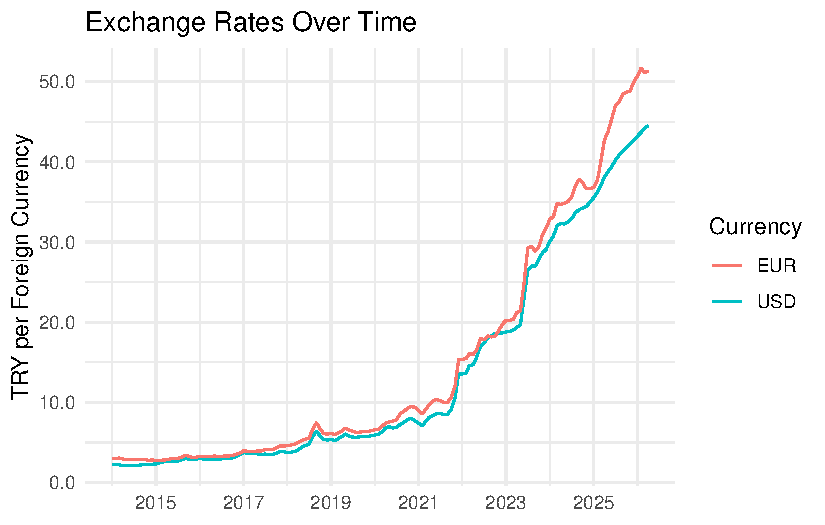
\includegraphics[keepaspectratio]{project_files/figure-pdf/unnamed-chunk-2-1.pdf}}
\end{itemize}

\subsubsection{Credit Card Expenditure
Table}\label{credit-card-expenditure-table}

\begin{itemize}
\item
  \textbf{Description}:
\item
  This table contains Year, Month, Expense Type, and Quantity.\\
\item
  Expense Type identifies the spending category, and Quantity gives the
  corresponding spending amount for that month.
\item
  This table contains sectoral spending amounts derived from credit card
  transactions.
\item
  The values in this table are expected to differ substantially across
  categories. Some categories such as retail, food, fuel, and e-commerce
  are likely to have much larger values than others.

\begin{Shaded}
\begin{Highlighting}[]
\FunctionTok{library}\NormalTok{(dplyr)}
\FunctionTok{library}\NormalTok{(ggplot2)}
\NormalTok{expense\_quantity }\OtherTok{\textless{}{-}}\NormalTok{ Expense\_Quantity }\SpecialCharTok{\%\textgreater{}\%}
  \FunctionTok{mutate}\NormalTok{(}\AttributeTok{Date =} \FunctionTok{as.Date}\NormalTok{(}\FunctionTok{sprintf}\NormalTok{(}\StringTok{"\%d{-}\%02d{-}01"}\NormalTok{, Year, Month)))}

\FunctionTok{ggplot}\NormalTok{(}
\NormalTok{  expense\_quantity }\SpecialCharTok{\%\textgreater{}\%}
    \FunctionTok{filter}\NormalTok{(Expense\_Type }\SpecialCharTok{\%in\%} \FunctionTok{c}\NormalTok{(}\StringTok{"E{-}Alışveriş"}\NormalTok{, }\StringTok{"Çeşitli Gıda"}\NormalTok{, }\StringTok{"Giyim ve Aksesuar"}\NormalTok{, }\StringTok{"Benzin ve Yakıt İstasyonları"}\NormalTok{)),}
  \FunctionTok{aes}\NormalTok{(}\AttributeTok{x =}\NormalTok{ Date, }\AttributeTok{y =}\NormalTok{ Quantity, }\AttributeTok{color =}\NormalTok{ Expense\_Type)}
\NormalTok{) }\SpecialCharTok{+}
  \FunctionTok{geom\_line}\NormalTok{() }\SpecialCharTok{+}
  \FunctionTok{labs}\NormalTok{(}
    \AttributeTok{title =} \StringTok{"Credit Card Expenditures for Selected Categories"}\NormalTok{,}
    \AttributeTok{x =} \StringTok{"Date"}\NormalTok{,}
    \AttributeTok{y =} \StringTok{"Quantity"}\NormalTok{,}
    \AttributeTok{color =} \StringTok{"Expense Type"}
\NormalTok{  ) }\SpecialCharTok{+}
  \FunctionTok{theme\_minimal}\NormalTok{()}
\end{Highlighting}
\end{Shaded}

  \pandocbounded{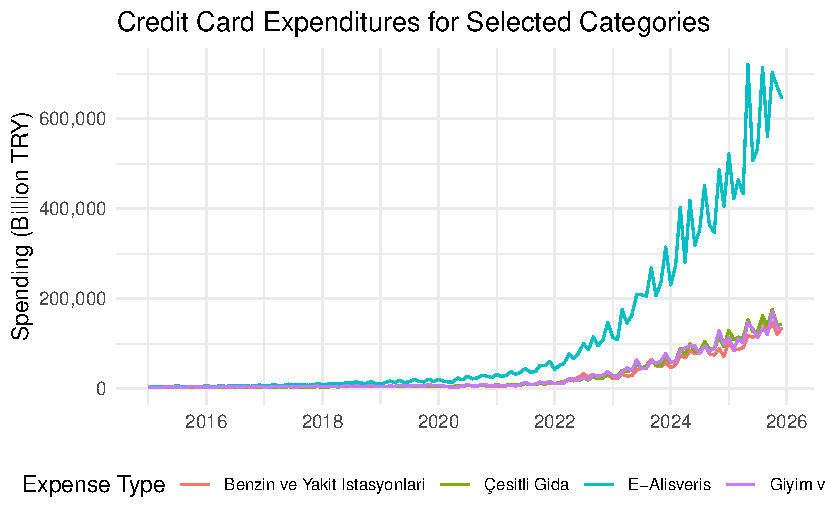
\includegraphics[keepaspectratio]{project_files/figure-pdf/unnamed-chunk-3-1.pdf}}
\end{itemize}

\subsubsection{Housing Panel Dataset}\label{housing-panel-dataset}

\begin{itemize}
\item
  \textbf{Description}:\\
  This is the main table for the project and contains Year, Month,
  Region, House Price Index, and Total Sales.

  Region represents the housing price index regions as in NUTS2 level,
  House Price Index shows the monthly house price index for that region,
  and Total Sales gives the aggregated monthly house sales value for the
  same region.

\begin{Shaded}
\begin{Highlighting}[]
\FunctionTok{library}\NormalTok{(dplyr)}
\FunctionTok{library}\NormalTok{(ggplot2)}

\NormalTok{konut\_index\_sales }\OtherTok{\textless{}{-}}\NormalTok{ Konut\_Index\_Sales }\SpecialCharTok{\%\textgreater{}\%}
  \FunctionTok{mutate}\NormalTok{(}\AttributeTok{Date =} \FunctionTok{as.Date}\NormalTok{(}\FunctionTok{sprintf}\NormalTok{(}\StringTok{"\%d{-}\%02d{-}01"}\NormalTok{, Year, Month)))}

\FunctionTok{ggplot}\NormalTok{(}
\NormalTok{  konut\_index\_sales }\SpecialCharTok{\%\textgreater{}\%} \FunctionTok{filter}\NormalTok{(Region }\SpecialCharTok{==} \StringTok{"Türkiye"}\NormalTok{),}
  \FunctionTok{aes}\NormalTok{(}\AttributeTok{x =}\NormalTok{ Date, }\AttributeTok{y =}\NormalTok{ Konut\_Endeksi)}
\NormalTok{) }\SpecialCharTok{+}
  \FunctionTok{geom\_line}\NormalTok{() }\SpecialCharTok{+}
  \FunctionTok{labs}\NormalTok{(}
    \AttributeTok{title =} \StringTok{"House Price Index in Türkiye Over Time"}\NormalTok{,}
    \AttributeTok{x =} \StringTok{"Date"}\NormalTok{,}
    \AttributeTok{y =} \StringTok{"House Price Index"}
\NormalTok{  ) }\SpecialCharTok{+}
  \FunctionTok{theme\_minimal}\NormalTok{()}
\end{Highlighting}
\end{Shaded}

  \pandocbounded{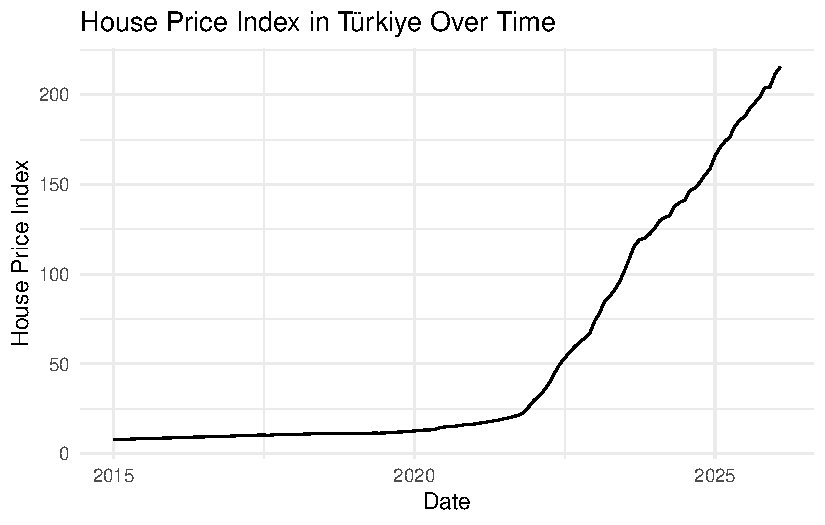
\includegraphics[keepaspectratio]{project_files/figure-pdf/unnamed-chunk-4-1.pdf}}
\end{itemize}

\begin{Shaded}
\begin{Highlighting}[]
\FunctionTok{library}\NormalTok{(dplyr)}
\FunctionTok{library}\NormalTok{(ggplot2)}

\FunctionTok{ggplot}\NormalTok{(}
\NormalTok{  Konut\_Index\_Sales }\SpecialCharTok{\%\textgreater{}\%}
    \FunctionTok{mutate}\NormalTok{(}\AttributeTok{Date =} \FunctionTok{as.Date}\NormalTok{(}\FunctionTok{sprintf}\NormalTok{(}\StringTok{"\%d{-}\%02d{-}01"}\NormalTok{, Year, Month))) }\SpecialCharTok{\%\textgreater{}\%}
    \FunctionTok{filter}\NormalTok{(Region }\SpecialCharTok{\%in\%} \FunctionTok{c}\NormalTok{(}\StringTok{"Türkiye"}\NormalTok{, }\StringTok{"İstanbul"}\NormalTok{, }\StringTok{"İzmir"}\NormalTok{, }\StringTok{"Ankara"}\NormalTok{, }\StringTok{"Adana, Mersin"}\NormalTok{)),}
  \FunctionTok{aes}\NormalTok{(}\AttributeTok{x =}\NormalTok{ Date, }\AttributeTok{y =}\NormalTok{ Total\_Sales, }\AttributeTok{color =}\NormalTok{ Region)}
\NormalTok{) }\SpecialCharTok{+}
  \FunctionTok{geom\_line}\NormalTok{() }\SpecialCharTok{+}
  \FunctionTok{labs}\NormalTok{(}
    \AttributeTok{title =} \StringTok{"Total House Sales for Selected Regions"}\NormalTok{,}
    \AttributeTok{x =} \StringTok{"Date"}\NormalTok{,}
    \AttributeTok{y =} \StringTok{"Total Sales"}\NormalTok{,}
    \AttributeTok{color =} \StringTok{"Region"}
\NormalTok{  ) }\SpecialCharTok{+}
  \FunctionTok{theme\_minimal}\NormalTok{()}
\end{Highlighting}
\end{Shaded}

\pandocbounded{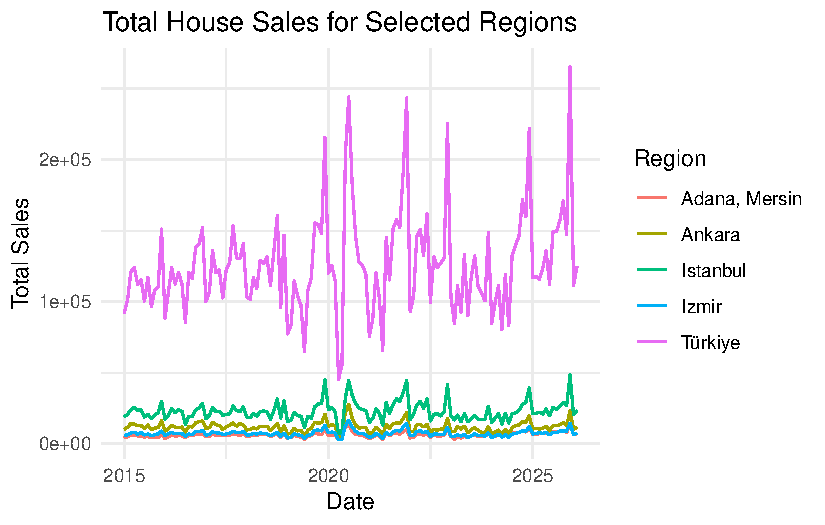
\includegraphics[keepaspectratio]{project_files/figure-pdf/unnamed-chunk-5-1.pdf}}

\subsection{Potential Analyses}\label{potential-analyses}

\begin{itemize}
\tightlist
\item
  time-series plots of house prices, exchange rates, and sales,
\item
  regional comparisons of house price growth,
\item
  correlations between exchange rates and the house price index,
\item
  relationships between sales volume and housing prices,
\item
  category-based spending trends over time,
\end{itemize}

\subsection{Reason of Choice}\label{reason-of-choice}

Housing prices are one of the most important economic and social issues
in Türkiye. The rapid increase in housing prices has significant
implications for affordability, investment decisions, and economic
stability.

All datasets are:

\begin{itemize}
\item
  Consistent in frequency (monthly)
\item
  Long enough for trend analysis
\item
  Rich enough for regional comparison

  This makes it easy for analyzing.
\end{itemize}

\subsection{Preprocessing}\label{preprocessing}

The raw EVDS datasets were provided in Excel format and contained
different structures (wide vs.~long) and aggregation levels (province
vs.~region). We performed preprocessing in Python using pandas to
standardize date formats, reshape wide datasets into long format, map
categorical codes to meaningful labels, and align all datasets at a
consistent monthly and regional level. In particular, house sales data
were converted from province-level columns to regional aggregates
compatible with the House Price Index. The final result consists of
three clean analytical tables ready for further analysis.

Another key issue was that EVDS datasets use \textbf{coded column names}
(e.g., \texttt{KT2}, \texttt{T58}, \texttt{TR62}) instead of descriptive
labels. To make the data interpretable and consistent across sources, we
created mapping dictionaries in Python to translate these codes into
meaningful categories, provinces, and regions.

Here you can find our python code.\\
\strut \\

\begin{Shaded}
\begin{Highlighting}[]
\CommentTok{\# We explained the data and the output tables to AI. It gave us this code\textquotesingle{}s first version. Then we fixed it according to our needs}
\ImportTok{import}\NormalTok{ pandas }\ImportTok{as}\NormalTok{ pd}
\ImportTok{from}\NormalTok{ pathlib }\ImportTok{import}\NormalTok{ Path}

\NormalTok{downloads }\OperatorTok{=}\NormalTok{ Path.home() }\OperatorTok{/} \StringTok{"Downloads"}

\CommentTok{\# Files}
\NormalTok{kurlar\_file }\OperatorTok{=}\NormalTok{ downloads }\OperatorTok{/} \StringTok{"Kurlar.xlsx"}
\NormalTok{kredi\_file }\OperatorTok{=}\NormalTok{ downloads }\OperatorTok{/} \StringTok{"Kredi Harcama.xlsx"}
\NormalTok{konut\_satis\_file }\OperatorTok{=}\NormalTok{ downloads }\OperatorTok{/} \StringTok{"Konut Satış.xlsx"}
\NormalTok{konut\_fiyat\_file }\OperatorTok{=}\NormalTok{ downloads }\OperatorTok{/} \StringTok{"Konut Fiyat Endexi.xlsx"}

\NormalTok{output\_file }\OperatorTok{=}\NormalTok{ downloads }\OperatorTok{/} \StringTok{"evds\_preprocessed\_tables\_fixed.xlsx"}

\CommentTok{\# {-}{-}{-}{-}{-}{-}{-}{-}{-}{-}{-}{-}{-}{-}{-}{-}{-}{-}{-}{-}{-}{-}{-}{-}{-}{-}{-}{-}{-}}
\CommentTok{\# Helper}
\CommentTok{\# {-}{-}{-}{-}{-}{-}{-}{-}{-}{-}{-}{-}{-}{-}{-}{-}{-}{-}{-}{-}{-}{-}{-}{-}{-}{-}{-}{-}{-}}
\KeywordTok{def}\NormalTok{ split\_year\_month(df):}
\NormalTok{    df[}\StringTok{"Tarih"}\NormalTok{] }\OperatorTok{=}\NormalTok{ pd.to\_datetime(df[}\StringTok{"Tarih"}\NormalTok{], }\BuiltInTok{format}\OperatorTok{=}\StringTok{"\%Y{-}\%m"}\NormalTok{)}
\NormalTok{    df[}\StringTok{"Year"}\NormalTok{] }\OperatorTok{=}\NormalTok{ df[}\StringTok{"Tarih"}\NormalTok{].dt.year}
\NormalTok{    df[}\StringTok{"Month"}\NormalTok{] }\OperatorTok{=}\NormalTok{ df[}\StringTok{"Tarih"}\NormalTok{].dt.month}
    \ControlFlowTok{return}\NormalTok{ df}

\CommentTok{\# {-}{-}{-}{-}{-}{-}{-}{-}{-}{-}{-}{-}{-}{-}{-}{-}{-}{-}{-}{-}{-}{-}{-}{-}{-}{-}{-}{-}{-}}
\CommentTok{\# Read}
\CommentTok{\# {-}{-}{-}{-}{-}{-}{-}{-}{-}{-}{-}{-}{-}{-}{-}{-}{-}{-}{-}{-}{-}{-}{-}{-}{-}{-}{-}{-}{-}}
\NormalTok{kurlar }\OperatorTok{=}\NormalTok{ split\_year\_month(pd.read\_excel(kurlar\_file))}
\NormalTok{kredi }\OperatorTok{=}\NormalTok{ split\_year\_month(pd.read\_excel(kredi\_file))}
\NormalTok{satis }\OperatorTok{=}\NormalTok{ split\_year\_month(pd.read\_excel(konut\_satis\_file))}
\NormalTok{kfe }\OperatorTok{=}\NormalTok{ split\_year\_month(pd.read\_excel(konut\_fiyat\_file))}

\CommentTok{\# {-}{-}{-}{-}{-}{-}{-}{-}{-}{-}{-}{-}{-}{-}{-}{-}{-}{-}{-}{-}{-}{-}{-}{-}{-}{-}{-}{-}{-}}
\CommentTok{\# TABLE 1: Exchange Rates}
\CommentTok{\# {-}{-}{-}{-}{-}{-}{-}{-}{-}{-}{-}{-}{-}{-}{-}{-}{-}{-}{-}{-}{-}{-}{-}{-}{-}{-}{-}{-}{-}}
\NormalTok{table\_kurlar }\OperatorTok{=}\NormalTok{ (}
\NormalTok{    kurlar[[}\StringTok{"Year"}\NormalTok{, }\StringTok{"Month"}\NormalTok{, }\StringTok{"TP\_DK\_USD\_S\_YTL"}\NormalTok{, }\StringTok{"TP\_DK\_EUR\_S\_YTL"}\NormalTok{]]}
\NormalTok{    .rename(columns}\OperatorTok{=}\NormalTok{\{}
        \StringTok{"TP\_DK\_USD\_S\_YTL"}\NormalTok{: }\StringTok{"USD"}\NormalTok{,}
        \StringTok{"TP\_DK\_EUR\_S\_YTL"}\NormalTok{: }\StringTok{"EUR"}
\NormalTok{    \})}
\NormalTok{)}

\CommentTok{\# {-}{-}{-}{-}{-}{-}{-}{-}{-}{-}{-}{-}{-}{-}{-}{-}{-}{-}{-}{-}{-}{-}{-}{-}{-}{-}{-}{-}{-}}
\CommentTok{\# TABLE 2: Credit Expenditures}
\CommentTok{\# {-}{-}{-}{-}{-}{-}{-}{-}{-}{-}{-}{-}{-}{-}{-}{-}{-}{-}{-}{-}{-}{-}{-}{-}{-}{-}{-}{-}{-}}
\NormalTok{expense\_type\_map }\OperatorTok{=}\NormalTok{ \{}
    \StringTok{"TP\_KKHARTUT\_KT2"}\NormalTok{: }\StringTok{"Car Rental"}\NormalTok{,}
    \StringTok{"TP\_KKHARTUT\_KT3"}\NormalTok{: }\StringTok{"Car Sales/Service"}\NormalTok{,}
    \StringTok{"TP\_KKHARTUT\_KT4"}\NormalTok{: }\StringTok{"Fuel"}\NormalTok{,}
    \StringTok{"TP\_KKHARTUT\_KT5"}\NormalTok{: }\StringTok{"Food"}\NormalTok{,}
    \StringTok{"TP\_KKHARTUT\_KT6"}\NormalTok{: }\StringTok{"Direct Marketing"}\NormalTok{,}
    \StringTok{"TP\_KKHARTUT\_KT7"}\NormalTok{: }\StringTok{"Education"}\NormalTok{,}
    \StringTok{"TP\_KKHARTUT\_KT8"}\NormalTok{: }\StringTok{"Electronics"}\NormalTok{,}
    \StringTok{"TP\_KKHARTUT\_KT9"}\NormalTok{: }\StringTok{"Clothing"}\NormalTok{,}
    \StringTok{"TP\_KKHARTUT\_KT10"}\NormalTok{: }\StringTok{"Airlines"}\NormalTok{,}
    \StringTok{"TP\_KKHARTUT\_KT11"}\NormalTok{: }\StringTok{"Services"}\NormalTok{,}
    \StringTok{"TP\_KKHARTUT\_KT12"}\NormalTok{: }\StringTok{"Accommodation"}\NormalTok{,}
    \StringTok{"TP\_KKHARTUT\_KT13"}\NormalTok{: }\StringTok{"Social"}\NormalTok{,}
    \StringTok{"TP\_KKHARTUT\_KT14"}\NormalTok{: }\StringTok{"Entertainment"}\NormalTok{,}
    \StringTok{"TP\_KKHARTUT\_KT15"}\NormalTok{: }\StringTok{"Jewelry"}\NormalTok{,}
    \StringTok{"TP\_KKHARTUT\_KT16"}\NormalTok{: }\StringTok{"Retail"}\NormalTok{,}
    \StringTok{"TP\_KKHARTUT\_KT17"}\NormalTok{: }\StringTok{"Furniture"}\NormalTok{,}
    \StringTok{"TP\_KKHARTUT\_KT18"}\NormalTok{: }\StringTok{"Construction"}\NormalTok{,}
    \StringTok{"TP\_KKHARTUT\_KT19"}\NormalTok{: }\StringTok{"Health"}\NormalTok{,}
    \StringTok{"TP\_KKHARTUT\_KT20"}\NormalTok{: }\StringTok{"Travel"}\NormalTok{,}
    \StringTok{"TP\_KKHARTUT\_KT21"}\NormalTok{: }\StringTok{"Insurance"}\NormalTok{,}
    \StringTok{"TP\_KKHARTUT\_KT22"}\NormalTok{: }\StringTok{"Telecom"}\NormalTok{,}
    \StringTok{"TP\_KKHARTUT\_KT23"}\NormalTok{: }\StringTok{"Hardware"}\NormalTok{,}
    \StringTok{"TP\_KKHARTUT\_KT24"}\NormalTok{: }\StringTok{"Food Service"}\NormalTok{,}
    \StringTok{"TP\_KKHARTUT\_KT25"}\NormalTok{: }\StringTok{"Misc"}\NormalTok{,}
    \StringTok{"TP\_KKHARTUT\_KT26"}\NormalTok{: }\StringTok{"Other"}\NormalTok{,}
    \StringTok{"TP\_KKHARTUT\_KT50"}\NormalTok{: }\StringTok{"E{-}Commerce"}
\NormalTok{\}}

\NormalTok{kredi\_cols }\OperatorTok{=}\NormalTok{ [c }\ControlFlowTok{for}\NormalTok{ c }\KeywordTok{in}\NormalTok{ expense\_type\_map }\ControlFlowTok{if}\NormalTok{ c }\KeywordTok{in}\NormalTok{ kredi.columns]}

\NormalTok{table\_kredi }\OperatorTok{=}\NormalTok{ (}
\NormalTok{    kredi.melt(}
\NormalTok{        id\_vars}\OperatorTok{=}\NormalTok{[}\StringTok{"Year"}\NormalTok{, }\StringTok{"Month"}\NormalTok{],}
\NormalTok{        value\_vars}\OperatorTok{=}\NormalTok{kredi\_cols,}
\NormalTok{        var\_name}\OperatorTok{=}\StringTok{"Code"}\NormalTok{,}
\NormalTok{        value\_name}\OperatorTok{=}\StringTok{"Quantity"}
\NormalTok{    )}
\NormalTok{    .assign(Expense\_Type}\OperatorTok{=}\KeywordTok{lambda}\NormalTok{ x: x[}\StringTok{"Code"}\NormalTok{].}\BuiltInTok{map}\NormalTok{(expense\_type\_map))}
\NormalTok{    [[}\StringTok{"Year"}\NormalTok{, }\StringTok{"Month"}\NormalTok{, }\StringTok{"Expense\_Type"}\NormalTok{, }\StringTok{"Quantity"}\NormalTok{]]}
\NormalTok{)}

\CommentTok{\# {-}{-}{-}{-}{-}{-}{-}{-}{-}{-}{-}{-}{-}{-}{-}{-}{-}{-}{-}{-}{-}{-}{-}{-}{-}{-}{-}{-}{-}}
\CommentTok{\# TABLE 3: Housing Panel}
\CommentTok{\# {-}{-}{-}{-}{-}{-}{-}{-}{-}{-}{-}{-}{-}{-}{-}{-}{-}{-}{-}{-}{-}{-}{-}{-}{-}{-}{-}{-}{-}}
\NormalTok{provinces }\OperatorTok{=}\NormalTok{ [}
    \StringTok{"Adana"}\NormalTok{,}\StringTok{"Adıyaman"}\NormalTok{,}\StringTok{"Afyonkarahisar"}\NormalTok{,}\StringTok{"Ağrı"}\NormalTok{,}\StringTok{"Aksaray"}\NormalTok{,}\StringTok{"Amasya"}\NormalTok{,}\StringTok{"Ankara"}\NormalTok{,}
    \StringTok{"Antalya"}\NormalTok{,}\StringTok{"Ardahan"}\NormalTok{,}\StringTok{"Artvin"}\NormalTok{,}\StringTok{"Aydın"}\NormalTok{,}\StringTok{"Balıkesir"}\NormalTok{,}\StringTok{"Bartın"}\NormalTok{,}\StringTok{"Batman"}\NormalTok{,}
    \StringTok{"Bayburt"}\NormalTok{,}\StringTok{"Bilecik"}\NormalTok{,}\StringTok{"Bingöl"}\NormalTok{,}\StringTok{"Bitlis"}\NormalTok{,}\StringTok{"Bolu"}\NormalTok{,}\StringTok{"Burdur"}\NormalTok{,}\StringTok{"Bursa"}\NormalTok{,}\StringTok{"Çanakkale"}\NormalTok{,}
    \StringTok{"Çankırı"}\NormalTok{,}\StringTok{"Çorum"}\NormalTok{,}\StringTok{"Denizli"}\NormalTok{,}\StringTok{"Diyarbakır"}\NormalTok{,}\StringTok{"Düzce"}\NormalTok{,}\StringTok{"Edirne"}\NormalTok{,}\StringTok{"Elazığ"}\NormalTok{,}
    \StringTok{"Erzincan"}\NormalTok{,}\StringTok{"Erzurum"}\NormalTok{,}\StringTok{"Eskişehir"}\NormalTok{,}\StringTok{"Gaziantep"}\NormalTok{,}\StringTok{"Giresun"}\NormalTok{,}\StringTok{"Gümüşhane"}\NormalTok{,}
    \StringTok{"Hakkâri"}\NormalTok{,}\StringTok{"Hatay"}\NormalTok{,}\StringTok{"Iğdır"}\NormalTok{,}\StringTok{"Isparta"}\NormalTok{,}\StringTok{"İstanbul"}\NormalTok{,}\StringTok{"İzmir"}\NormalTok{,}\StringTok{"Kahramanmaraş"}\NormalTok{,}
    \StringTok{"Karabük"}\NormalTok{,}\StringTok{"Karaman"}\NormalTok{,}\StringTok{"Kars"}\NormalTok{,}\StringTok{"Kastamonu"}\NormalTok{,}\StringTok{"Kayseri"}\NormalTok{,}\StringTok{"Kırıkkale"}\NormalTok{,}\StringTok{"Kırklareli"}\NormalTok{,}
    \StringTok{"Kırşehir"}\NormalTok{,}\StringTok{"Kilis"}\NormalTok{,}\StringTok{"Kocaeli"}\NormalTok{,}\StringTok{"Konya"}\NormalTok{,}\StringTok{"Kütahya"}\NormalTok{,}\StringTok{"Malatya"}\NormalTok{,}\StringTok{"Manisa"}\NormalTok{,}
    \StringTok{"Mardin"}\NormalTok{,}\StringTok{"Mersin"}\NormalTok{,}\StringTok{"Muğla"}\NormalTok{,}\StringTok{"Muş"}\NormalTok{,}\StringTok{"Nevşehir"}\NormalTok{,}\StringTok{"Niğde"}\NormalTok{,}\StringTok{"Ordu"}\NormalTok{,}\StringTok{"Osmaniye"}\NormalTok{,}
    \StringTok{"Rize"}\NormalTok{,}\StringTok{"Sakarya"}\NormalTok{,}\StringTok{"Samsun"}\NormalTok{,}\StringTok{"Siirt"}\NormalTok{,}\StringTok{"Sinop"}\NormalTok{,}\StringTok{"Sivas"}\NormalTok{,}\StringTok{"Şanlıurfa"}\NormalTok{,}\StringTok{"Şırnak"}\NormalTok{,}
    \StringTok{"Tekirdağ"}\NormalTok{,}\StringTok{"Tokat"}\NormalTok{,}\StringTok{"Trabzon"}\NormalTok{,}\StringTok{"Tunceli"}\NormalTok{,}\StringTok{"Uşak"}\NormalTok{,}\StringTok{"Van"}\NormalTok{,}\StringTok{"Yalova"}\NormalTok{,}\StringTok{"Yozgat"}\NormalTok{,}
    \StringTok{"Zonguldak"}
\NormalTok{]}

\NormalTok{code\_map }\OperatorTok{=}\NormalTok{ \{}\StringTok{"TP\_AKONUTSAT1\_K1"}\NormalTok{: provinces[}\DecValTok{0}\NormalTok{]\}}
\ControlFlowTok{for}\NormalTok{ i }\KeywordTok{in} \BuiltInTok{range}\NormalTok{(}\DecValTok{2}\NormalTok{, }\DecValTok{82}\NormalTok{):}
\NormalTok{    code\_map[}\SpecialStringTok{f"TP\_AKONUTSAT1\_T}\SpecialCharTok{\{}\NormalTok{i}\SpecialCharTok{\}}\SpecialStringTok{"}\NormalTok{] }\OperatorTok{=}\NormalTok{ provinces[i}\OperatorTok{{-}}\DecValTok{1}\NormalTok{]}

\NormalTok{sales\_cols }\OperatorTok{=}\NormalTok{ [c }\ControlFlowTok{for}\NormalTok{ c }\KeywordTok{in}\NormalTok{ satis.columns }\ControlFlowTok{if}\NormalTok{ c }\KeywordTok{in}\NormalTok{ code\_map]}

\NormalTok{sales\_long }\OperatorTok{=}\NormalTok{ (}
\NormalTok{    satis.melt(}
\NormalTok{        id\_vars}\OperatorTok{=}\NormalTok{[}\StringTok{"Year"}\NormalTok{, }\StringTok{"Month"}\NormalTok{],}
\NormalTok{        value\_vars}\OperatorTok{=}\NormalTok{sales\_cols,}
\NormalTok{        var\_name}\OperatorTok{=}\StringTok{"Code"}\NormalTok{,}
\NormalTok{        value\_name}\OperatorTok{=}\StringTok{"Sales"}
\NormalTok{    )}
\NormalTok{    .assign(Province}\OperatorTok{=}\KeywordTok{lambda}\NormalTok{ x: x[}\StringTok{"Code"}\NormalTok{].}\BuiltInTok{map}\NormalTok{(code\_map))}
\NormalTok{)}

\CommentTok{\# Region mapping (example simplified)}
\NormalTok{region\_map }\OperatorTok{=}\NormalTok{ \{}
    \StringTok{"Adana"}\NormalTok{:}\StringTok{"TR62"}\NormalTok{,}\StringTok{"Mersin"}\NormalTok{:}\StringTok{"TR62"}\NormalTok{,}\StringTok{"Ankara"}\NormalTok{:}\StringTok{"TR51"}\NormalTok{,}\StringTok{"İstanbul"}\NormalTok{:}\StringTok{"TR10"}
\NormalTok{\}}

\NormalTok{sales\_long[}\StringTok{"Region\_Code"}\NormalTok{] }\OperatorTok{=}\NormalTok{ sales\_long[}\StringTok{"Province"}\NormalTok{].}\BuiltInTok{map}\NormalTok{(region\_map)}

\NormalTok{sales\_region }\OperatorTok{=}\NormalTok{ (}
\NormalTok{    sales\_long.groupby([}\StringTok{"Year"}\NormalTok{,}\StringTok{"Month"}\NormalTok{,}\StringTok{"Region\_Code"}\NormalTok{])[}\StringTok{"Sales"}\NormalTok{].}\BuiltInTok{sum}\NormalTok{().reset\_index()}
\NormalTok{)}

\NormalTok{kfe\_map }\OperatorTok{=}\NormalTok{ \{}
    \StringTok{"TP\_KFE\_TR62"}\NormalTok{:}\StringTok{"TR62"}\NormalTok{,}
    \StringTok{"TP\_KFE\_TR51"}\NormalTok{:}\StringTok{"TR51"}\NormalTok{,}
    \StringTok{"TP\_KFE\_TR10"}\NormalTok{:}\StringTok{"TR10"}
\NormalTok{\}}

\NormalTok{kfe\_cols }\OperatorTok{=}\NormalTok{ [c }\ControlFlowTok{for}\NormalTok{ c }\KeywordTok{in}\NormalTok{ kfe\_map }\ControlFlowTok{if}\NormalTok{ c }\KeywordTok{in}\NormalTok{ kfe.columns]}

\NormalTok{kfe\_long }\OperatorTok{=}\NormalTok{ (}
\NormalTok{    kfe.melt(}
\NormalTok{        id\_vars}\OperatorTok{=}\NormalTok{[}\StringTok{"Year"}\NormalTok{,}\StringTok{"Month"}\NormalTok{],}
\NormalTok{        value\_vars}\OperatorTok{=}\NormalTok{kfe\_cols,}
\NormalTok{        var\_name}\OperatorTok{=}\StringTok{"Code"}\NormalTok{,}
\NormalTok{        value\_name}\OperatorTok{=}\StringTok{"House\_Price\_Index"}
\NormalTok{    )}
\NormalTok{    .assign(Region\_Code}\OperatorTok{=}\KeywordTok{lambda}\NormalTok{ x: x[}\StringTok{"Code"}\NormalTok{].}\BuiltInTok{map}\NormalTok{(kfe\_map))}
\NormalTok{)}

\NormalTok{table\_konut }\OperatorTok{=}\NormalTok{ kfe\_long.merge(}
\NormalTok{    sales\_region,}
\NormalTok{    on}\OperatorTok{=}\NormalTok{[}\StringTok{"Year"}\NormalTok{,}\StringTok{"Month"}\NormalTok{,}\StringTok{"Region\_Code"}\NormalTok{]}
\NormalTok{)}

\CommentTok{\# {-}{-}{-}{-}{-}{-}{-}{-}{-}{-}{-}{-}{-}{-}{-}{-}{-}{-}{-}{-}{-}{-}{-}{-}{-}{-}{-}{-}{-}}
\CommentTok{\# SAVE}
\CommentTok{\# {-}{-}{-}{-}{-}{-}{-}{-}{-}{-}{-}{-}{-}{-}{-}{-}{-}{-}{-}{-}{-}{-}{-}{-}{-}{-}{-}{-}{-}}
\ControlFlowTok{with}\NormalTok{ pd.ExcelWriter(output\_file) }\ImportTok{as}\NormalTok{ writer:}
\NormalTok{    table\_kurlar.to\_excel(writer, sheet\_name}\OperatorTok{=}\StringTok{"USD\_EUR"}\NormalTok{, index}\OperatorTok{=}\VariableTok{False}\NormalTok{)}
\NormalTok{    table\_kredi.to\_excel(writer, sheet\_name}\OperatorTok{=}\StringTok{"Expense"}\NormalTok{, index}\OperatorTok{=}\VariableTok{False}\NormalTok{)}
\NormalTok{    table\_konut.to\_excel(writer, sheet\_name}\OperatorTok{=}\StringTok{"Housing"}\NormalTok{, index}\OperatorTok{=}\VariableTok{False}\NormalTok{)}
\end{Highlighting}
\end{Shaded}

\section{Analysis}\label{analysis}

This section presents the full analytical workflow: exploratory data
analysis, trend decomposition, correlation analysis, regional
comparison, and predictive modelling. All code is collapsible for
readability; outputs and narrative explanations accompany each step.

\subsection{Exploratory Data Analysis}\label{exploratory-data-analysis}

We begin by loading the data and performing a structured overview of
each of the three tables.

\begin{Shaded}
\begin{Highlighting}[]
\FunctionTok{library}\NormalTok{(dplyr)}
\FunctionTok{library}\NormalTok{(ggplot2)}
\FunctionTok{library}\NormalTok{(tidyr)}
\FunctionTok{library}\NormalTok{(scales)}
\FunctionTok{library}\NormalTok{(knitr)}
\FunctionTok{library}\NormalTok{(kableExtra)}

\CommentTok{\# Load data}
\FunctionTok{load}\NormalTok{(}\StringTok{"Project\_Data.RData"}\NormalTok{)}

\CommentTok{\# Build date columns}
\NormalTok{cr }\OtherTok{\textless{}{-}}\NormalTok{ Conversion\_Rates }\SpecialCharTok{\%\textgreater{}\%}
  \FunctionTok{mutate}\NormalTok{(}\AttributeTok{Date =} \FunctionTok{as.Date}\NormalTok{(}\FunctionTok{sprintf}\NormalTok{(}\StringTok{"\%d{-}\%02d{-}01"}\NormalTok{, Year, Month)))}

\NormalTok{eq }\OtherTok{\textless{}{-}}\NormalTok{ Expense\_Quantity }\SpecialCharTok{\%\textgreater{}\%}
  \FunctionTok{mutate}\NormalTok{(}\AttributeTok{Date =} \FunctionTok{as.Date}\NormalTok{(}\FunctionTok{sprintf}\NormalTok{(}\StringTok{"\%d{-}\%02d{-}01"}\NormalTok{, Year, Month)))}

\NormalTok{ks }\OtherTok{\textless{}{-}}\NormalTok{ Konut\_Index\_Sales }\SpecialCharTok{\%\textgreater{}\%}
  \FunctionTok{mutate}\NormalTok{(}\AttributeTok{Date =} \FunctionTok{as.Date}\NormalTok{(}\FunctionTok{sprintf}\NormalTok{(}\StringTok{"\%d{-}\%02d{-}01"}\NormalTok{, Year, Month)))}
\end{Highlighting}
\end{Shaded}

\subsubsection{Summary Statistics}\label{summary-statistics}

\paragraph{Exchange Rates}\label{exchange-rates}

\begin{Shaded}
\begin{Highlighting}[]
\NormalTok{cr\_summary }\OtherTok{\textless{}{-}}\NormalTok{ cr }\SpecialCharTok{\%\textgreater{}\%}
  \FunctionTok{select}\NormalTok{(USD, EUR) }\SpecialCharTok{\%\textgreater{}\%}
  \FunctionTok{summarise}\NormalTok{(}
    \FunctionTok{across}\NormalTok{(}\FunctionTok{everything}\NormalTok{(), }\FunctionTok{list}\NormalTok{(}
      \AttributeTok{Min    =}\NormalTok{ min,}
      \AttributeTok{Mean   =}\NormalTok{ mean,}
      \AttributeTok{Median =}\NormalTok{ median,}
      \AttributeTok{Max    =}\NormalTok{ max,}
      \AttributeTok{SD     =}\NormalTok{ sd}
\NormalTok{    ), }\AttributeTok{.names =} \StringTok{"\{.col\}\_\{.fn\}"}\NormalTok{)}
\NormalTok{  ) }\SpecialCharTok{\%\textgreater{}\%}
  \FunctionTok{pivot\_longer}\NormalTok{(}\FunctionTok{everything}\NormalTok{(), }\AttributeTok{names\_to =} \FunctionTok{c}\NormalTok{(}\StringTok{"Currency"}\NormalTok{, }\StringTok{"Stat"}\NormalTok{), }\AttributeTok{names\_sep =} \StringTok{"\_"}\NormalTok{) }\SpecialCharTok{\%\textgreater{}\%}
  \FunctionTok{pivot\_wider}\NormalTok{(}\AttributeTok{names\_from =}\NormalTok{ Stat, }\AttributeTok{values\_from =}\NormalTok{ value)}

\FunctionTok{kable}\NormalTok{(cr\_summary, }\AttributeTok{digits =} \DecValTok{2}\NormalTok{, }\AttributeTok{caption =} \StringTok{"Summary Statistics – Exchange Rates (TRY)"}\NormalTok{) }\SpecialCharTok{\%\textgreater{}\%}
  \FunctionTok{kable\_styling}\NormalTok{(}\AttributeTok{bootstrap\_options =} \FunctionTok{c}\NormalTok{(}\StringTok{"striped"}\NormalTok{, }\StringTok{"hover"}\NormalTok{), }\AttributeTok{full\_width =} \ConstantTok{FALSE}\NormalTok{)}
\end{Highlighting}
\end{Shaded}

\begin{longtable}[t]{lrrrrr}
\caption{\label{tab:eda-exchange-summary}Summary Statistics – Exchange Rates (TRY)}\\
\toprule
Currency & Min & Mean & Median & Max & SD\\
\midrule
USD & 2.09 & 13.40 & 6.35 & 44.49 & 13.26\\
EUR & 2.72 & 14.94 & 7.22 & 51.68 & 14.80\\
\bottomrule
\end{longtable}

The USD/TRY rate grew from a minimum near 2 TRY to over 30 TRY across
the sample period, illustrating the scale of currency depreciation. The
EUR/TRY series followed a similar trajectory. The high standard
deviations relative to means confirm that these series are strongly
trended rather than stationary.

\paragraph{House Price Index and Sales
(National)}\label{house-price-index-and-sales-national}

\begin{Shaded}
\begin{Highlighting}[]
\NormalTok{ks\_turkey }\OtherTok{\textless{}{-}}\NormalTok{ ks }\SpecialCharTok{\%\textgreater{}\%} \FunctionTok{filter}\NormalTok{(Region }\SpecialCharTok{==} \StringTok{"Türkiye"}\NormalTok{)}

\NormalTok{hpi\_summary }\OtherTok{\textless{}{-}}\NormalTok{ ks\_turkey }\SpecialCharTok{\%\textgreater{}\%}
  \FunctionTok{summarise}\NormalTok{(}
    \AttributeTok{N          =} \FunctionTok{n}\NormalTok{(),}
    \AttributeTok{HPI\_Min    =} \FunctionTok{min}\NormalTok{(Konut\_Endeksi, }\AttributeTok{na.rm =} \ConstantTok{TRUE}\NormalTok{),}
    \AttributeTok{HPI\_Mean   =} \FunctionTok{mean}\NormalTok{(Konut\_Endeksi, }\AttributeTok{na.rm =} \ConstantTok{TRUE}\NormalTok{),}
    \AttributeTok{HPI\_Median =} \FunctionTok{median}\NormalTok{(Konut\_Endeksi, }\AttributeTok{na.rm =} \ConstantTok{TRUE}\NormalTok{),}
    \AttributeTok{HPI\_Max    =} \FunctionTok{max}\NormalTok{(Konut\_Endeksi, }\AttributeTok{na.rm =} \ConstantTok{TRUE}\NormalTok{),}
    \AttributeTok{HPI\_SD     =} \FunctionTok{sd}\NormalTok{(Konut\_Endeksi, }\AttributeTok{na.rm =} \ConstantTok{TRUE}\NormalTok{),}
    \AttributeTok{Sales\_Min  =} \FunctionTok{min}\NormalTok{(Total\_Sales, }\AttributeTok{na.rm =} \ConstantTok{TRUE}\NormalTok{),}
    \AttributeTok{Sales\_Mean =} \FunctionTok{mean}\NormalTok{(Total\_Sales, }\AttributeTok{na.rm =} \ConstantTok{TRUE}\NormalTok{),}
    \AttributeTok{Sales\_Max  =} \FunctionTok{max}\NormalTok{(Total\_Sales, }\AttributeTok{na.rm =} \ConstantTok{TRUE}\NormalTok{),}
    \AttributeTok{Sales\_SD   =} \FunctionTok{sd}\NormalTok{(Total\_Sales, }\AttributeTok{na.rm =} \ConstantTok{TRUE}\NormalTok{)}
\NormalTok{  )}

\FunctionTok{kable}\NormalTok{(}\FunctionTok{t}\NormalTok{(hpi\_summary), }\AttributeTok{col.names =} \StringTok{"Value"}\NormalTok{, }\AttributeTok{caption =} \StringTok{"Summary – National HPI and Sales"}\NormalTok{) }\SpecialCharTok{\%\textgreater{}\%}
  \FunctionTok{kable\_styling}\NormalTok{(}\AttributeTok{bootstrap\_options =} \FunctionTok{c}\NormalTok{(}\StringTok{"striped"}\NormalTok{), }\AttributeTok{full\_width =} \ConstantTok{FALSE}\NormalTok{)}
\end{Highlighting}
\end{Shaded}

\begin{longtable}[t]{lr}
\caption{\label{tab:eda-hpi-summary}Summary – National HPI and Sales}\\
\toprule
 & Value\\
\midrule
N & 134.00000\\
HPI\_Min & 7.65000\\
HPI\_Mean & 53.52418\\
HPI\_Median & 14.95500\\
HPI\_Max & 215.51000\\
\addlinespace
HPI\_SD & 63.49457\\
Sales\_Min & 45218.00000\\
Sales\_Mean & 126019.36567\\
Sales\_Max & 265223.00000\\
Sales\_SD & 35471.83237\\
\bottomrule
\end{longtable}

The national HPI has grown dramatically, with the maximum value being
many multiples of the minimum. Sales volumes display high variability,
reflecting seasonal patterns and market shifts.

\paragraph{Credit Card Expenditure (Top
Categories)}\label{credit-card-expenditure-top-categories}

\begin{Shaded}
\begin{Highlighting}[]
\NormalTok{top\_cats }\OtherTok{\textless{}{-}}\NormalTok{ eq }\SpecialCharTok{\%\textgreater{}\%}
  \FunctionTok{group\_by}\NormalTok{(Expense\_Type) }\SpecialCharTok{\%\textgreater{}\%}
  \FunctionTok{summarise}\NormalTok{(}\AttributeTok{Total =} \FunctionTok{sum}\NormalTok{(Quantity, }\AttributeTok{na.rm =} \ConstantTok{TRUE}\NormalTok{)) }\SpecialCharTok{\%\textgreater{}\%}
  \FunctionTok{arrange}\NormalTok{(}\FunctionTok{desc}\NormalTok{(Total)) }\SpecialCharTok{\%\textgreater{}\%}
  \FunctionTok{slice\_head}\NormalTok{(}\AttributeTok{n =} \DecValTok{8}\NormalTok{)}

\FunctionTok{kable}\NormalTok{(top\_cats, }\AttributeTok{digits =} \DecValTok{0}\NormalTok{,}
      \AttributeTok{col.names =} \FunctionTok{c}\NormalTok{(}\StringTok{"Expense Category"}\NormalTok{, }\StringTok{"Total Spending (Million TRY)"}\NormalTok{),}
      \AttributeTok{caption =} \StringTok{"Top 8 Credit Card Expenditure Categories (Cumulative)"}\NormalTok{) }\SpecialCharTok{\%\textgreater{}\%}
  \FunctionTok{kable\_styling}\NormalTok{(}\AttributeTok{bootstrap\_options =} \FunctionTok{c}\NormalTok{(}\StringTok{"striped"}\NormalTok{, }\StringTok{"hover"}\NormalTok{), }\AttributeTok{full\_width =} \ConstantTok{FALSE}\NormalTok{)}
\end{Highlighting}
\end{Shaded}

\begin{longtable}[t]{lr}
\caption{\label{tab:eda-credit-summary}Top 8 Credit Card Expenditure Categories (Cumulative)}\\
\toprule
Expense Category & Total Spending (Million TRY)\\
\midrule
E-Alışveriş & 17938599003\\
Market ve Alışveriş Merkezleri & 11837257322\\
Çeşitli Gıda & 4395417545\\
Giyim ve Aksesuar & 4315131168\\
Benzin ve Yakıt İstasyonları & 3932543095\\
\addlinespace
Hizmet Sektörleri & 3891104522\\
Elektrik-Elektronik Eşya / Bilgisayar & 3585052672\\
Çeşitli & 3572937540\\
\bottomrule
\end{longtable}

Retail trade, food, and e-commerce consistently rank as the largest
credit card spending categories. Furniture and construction-related
categories, while smaller in absolute terms, are of particular interest
given their direct linkage to the housing market.

\subsubsection{Distribution Analysis}\label{distribution-analysis}

\begin{Shaded}
\begin{Highlighting}[]
\NormalTok{p1 }\OtherTok{\textless{}{-}} \FunctionTok{ggplot}\NormalTok{(ks\_turkey, }\FunctionTok{aes}\NormalTok{(}\AttributeTok{x =}\NormalTok{ Konut\_Endeksi)) }\SpecialCharTok{+}
  \FunctionTok{geom\_histogram}\NormalTok{(}\AttributeTok{bins =} \DecValTok{30}\NormalTok{, }\AttributeTok{fill =} \StringTok{"\#2c7bb6"}\NormalTok{, }\AttributeTok{color =} \StringTok{"white"}\NormalTok{, }\AttributeTok{alpha =} \FloatTok{0.85}\NormalTok{) }\SpecialCharTok{+}
  \FunctionTok{labs}\NormalTok{(}\AttributeTok{title =} \StringTok{"HPI Distribution"}\NormalTok{, }\AttributeTok{x =} \StringTok{"House Price Index"}\NormalTok{, }\AttributeTok{y =} \StringTok{"Count"}\NormalTok{) }\SpecialCharTok{+}
  \FunctionTok{theme\_minimal}\NormalTok{()}

\NormalTok{p2 }\OtherTok{\textless{}{-}} \FunctionTok{ggplot}\NormalTok{(cr, }\FunctionTok{aes}\NormalTok{(}\AttributeTok{x =}\NormalTok{ USD)) }\SpecialCharTok{+}
  \FunctionTok{geom\_histogram}\NormalTok{(}\AttributeTok{bins =} \DecValTok{30}\NormalTok{, }\AttributeTok{fill =} \StringTok{"\#d7191c"}\NormalTok{, }\AttributeTok{color =} \StringTok{"white"}\NormalTok{, }\AttributeTok{alpha =} \FloatTok{0.85}\NormalTok{) }\SpecialCharTok{+}
  \FunctionTok{labs}\NormalTok{(}\AttributeTok{title =} \StringTok{"USD/TRY Distribution"}\NormalTok{, }\AttributeTok{x =} \StringTok{"USD Rate"}\NormalTok{, }\AttributeTok{y =} \StringTok{"Count"}\NormalTok{) }\SpecialCharTok{+}
  \FunctionTok{theme\_minimal}\NormalTok{()}

\FunctionTok{library}\NormalTok{(patchwork)}
\NormalTok{p1 }\SpecialCharTok{+}\NormalTok{ p2}
\end{Highlighting}
\end{Shaded}

\begin{figure}[H]

{\centering \pandocbounded{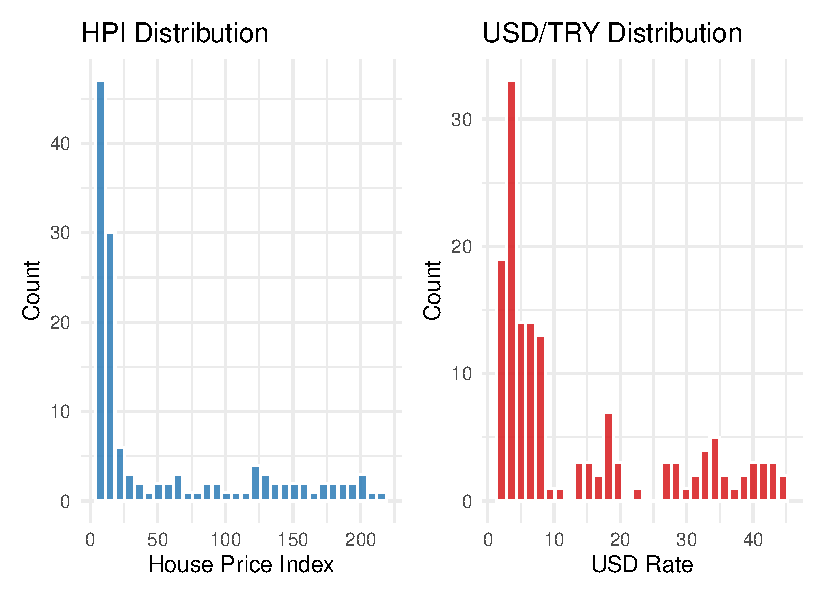
\includegraphics[keepaspectratio]{project_files/figure-pdf/eda-distributions-1.pdf}}

}

\caption{Distribution of key variables}

\end{figure}%

Both the HPI and the exchange rate show right-skewed, strongly
non-normal distributions --- a natural consequence of exponential growth
trajectories. This motivates the use of log-transformations in the
regression modelling step.

\subsection{Trend Analysis}\label{trend-analysis}

\subsubsection{House Price Index -- National
Trend}\label{house-price-index-national-trend}

\begin{Shaded}
\begin{Highlighting}[]
\FunctionTok{ggplot}\NormalTok{(ks\_turkey, }\FunctionTok{aes}\NormalTok{(}\AttributeTok{x =}\NormalTok{ Date, }\AttributeTok{y =}\NormalTok{ Konut\_Endeksi)) }\SpecialCharTok{+}
  \FunctionTok{geom\_line}\NormalTok{(}\AttributeTok{color =} \StringTok{"\#2c7bb6"}\NormalTok{, }\AttributeTok{linewidth =} \FloatTok{0.9}\NormalTok{) }\SpecialCharTok{+}
  \FunctionTok{geom\_smooth}\NormalTok{(}\AttributeTok{method =} \StringTok{"loess"}\NormalTok{, }\AttributeTok{se =} \ConstantTok{TRUE}\NormalTok{, }\AttributeTok{color =} \StringTok{"\#d7191c"}\NormalTok{,}
              \AttributeTok{fill =} \StringTok{"\#fdae61"}\NormalTok{, }\AttributeTok{alpha =} \FloatTok{0.25}\NormalTok{, }\AttributeTok{linewidth =} \FloatTok{0.8}\NormalTok{) }\SpecialCharTok{+}
  \FunctionTok{scale\_y\_continuous}\NormalTok{(}\AttributeTok{labels =}\NormalTok{ comma) }\SpecialCharTok{+}
  \FunctionTok{labs}\NormalTok{(}
    \AttributeTok{title    =} \StringTok{"National House Price Index Over Time"}\NormalTok{,}
    \AttributeTok{subtitle =} \StringTok{"Monthly data from TCMB{-}EVDS; LOESS trend overlay"}\NormalTok{,}
    \AttributeTok{x =} \StringTok{"Date"}\NormalTok{, }\AttributeTok{y =} \StringTok{"House Price Index"}
\NormalTok{  ) }\SpecialCharTok{+}
  \FunctionTok{theme\_minimal}\NormalTok{(}\AttributeTok{base\_size =} \DecValTok{11}\NormalTok{)}
\end{Highlighting}
\end{Shaded}

\begin{figure}[H]

{\centering \pandocbounded{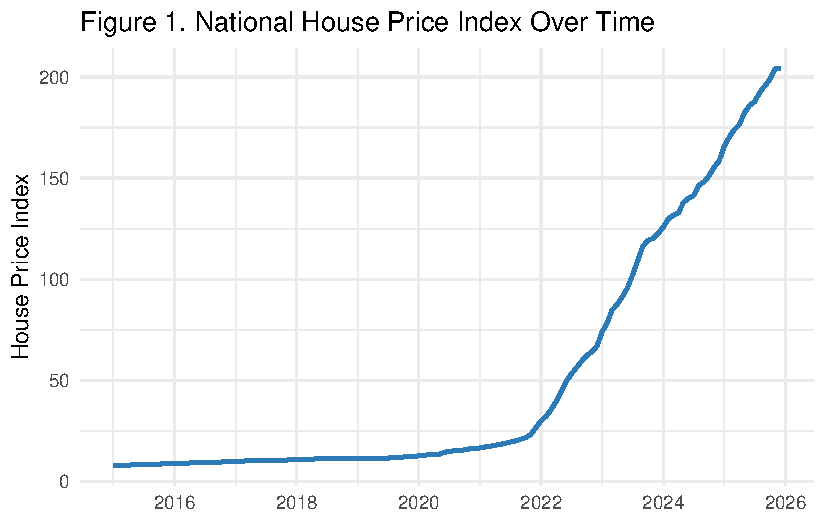
\includegraphics[keepaspectratio]{project_files/figure-pdf/trend-hpi-1.pdf}}

}

\caption{National House Price Index (2014--2024) with trend line}

\end{figure}%

The national HPI shows a gradual increase through 2019, followed by an
accelerating surge from 2020 onward. Three distinct phases are visible:
a moderate growth phase (2014--2019), an early acceleration phase
(2020--2021), and a sharp exponential surge (2022--2024), closely
coinciding with episodes of severe TRY depreciation.

\subsubsection{Exchange Rate Trends}\label{exchange-rate-trends}

\begin{Shaded}
\begin{Highlighting}[]
\NormalTok{cr\_long }\OtherTok{\textless{}{-}}\NormalTok{ cr }\SpecialCharTok{\%\textgreater{}\%}
  \FunctionTok{pivot\_longer}\NormalTok{(}\AttributeTok{cols =} \FunctionTok{c}\NormalTok{(USD, EUR), }\AttributeTok{names\_to =} \StringTok{"Currency"}\NormalTok{, }\AttributeTok{values\_to =} \StringTok{"Rate"}\NormalTok{)}

\FunctionTok{ggplot}\NormalTok{(cr\_long, }\FunctionTok{aes}\NormalTok{(}\AttributeTok{x =}\NormalTok{ Date, }\AttributeTok{y =}\NormalTok{ Rate, }\AttributeTok{color =}\NormalTok{ Currency)) }\SpecialCharTok{+}
  \FunctionTok{geom\_line}\NormalTok{(}\AttributeTok{linewidth =} \FloatTok{0.9}\NormalTok{) }\SpecialCharTok{+}
  \FunctionTok{scale\_color\_manual}\NormalTok{(}\AttributeTok{values =} \FunctionTok{c}\NormalTok{(}\StringTok{"USD"} \OtherTok{=} \StringTok{"\#2c7bb6"}\NormalTok{, }\StringTok{"EUR"} \OtherTok{=} \StringTok{"\#1a9641"}\NormalTok{)) }\SpecialCharTok{+}
  \FunctionTok{scale\_y\_continuous}\NormalTok{(}\AttributeTok{labels =}\NormalTok{ comma) }\SpecialCharTok{+}
  \FunctionTok{labs}\NormalTok{(}
    \AttributeTok{title    =} \StringTok{"Exchange Rate Movements (USD/TRY, EUR/TRY)"}\NormalTok{,}
    \AttributeTok{subtitle =} \StringTok{"Data source: TCMB{-}EVDS"}\NormalTok{,}
    \AttributeTok{x =} \StringTok{"Date"}\NormalTok{, }\AttributeTok{y =} \StringTok{"TRY per Foreign Currency"}
\NormalTok{  ) }\SpecialCharTok{+}
  \FunctionTok{theme\_minimal}\NormalTok{(}\AttributeTok{base\_size =} \DecValTok{11}\NormalTok{)}
\end{Highlighting}
\end{Shaded}

\begin{figure}[H]

{\centering \pandocbounded{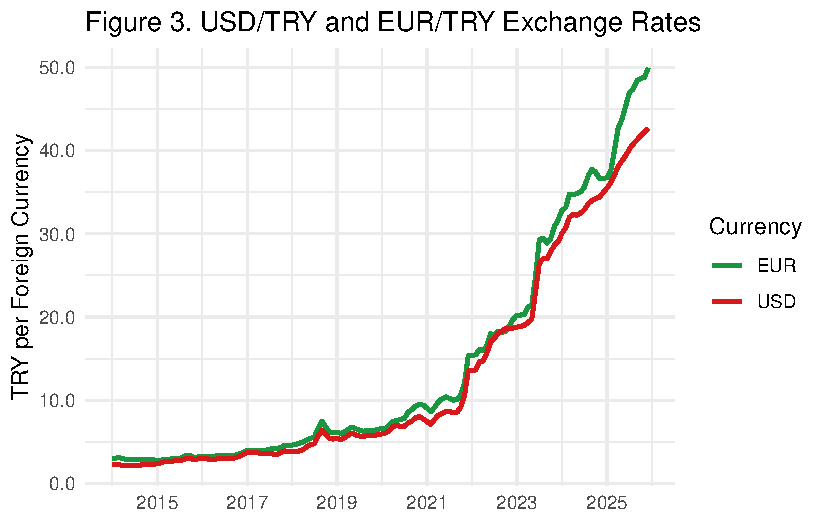
\includegraphics[keepaspectratio]{project_files/figure-pdf/trend-fx-1.pdf}}

}

\caption{USD/TRY and EUR/TRY exchange rates over time}

\end{figure}%

Both rates track each other closely and display the same phase structure
as the HPI, providing initial visual evidence of co-movement. The
sharpest depreciations occurred in 2021--2022 and again in 2023,
corresponding directly to the most aggressive phases of HPI growth.

\subsubsection{Housing Sales Trend}\label{housing-sales-trend}

\begin{Shaded}
\begin{Highlighting}[]
\NormalTok{ks\_turkey\_ma }\OtherTok{\textless{}{-}}\NormalTok{ ks\_turkey }\SpecialCharTok{\%\textgreater{}\%}
  \FunctionTok{arrange}\NormalTok{(Date) }\SpecialCharTok{\%\textgreater{}\%}
  \FunctionTok{mutate}\NormalTok{(}\AttributeTok{MA12 =}\NormalTok{ zoo}\SpecialCharTok{::}\FunctionTok{rollmean}\NormalTok{(Total\_Sales, }\AttributeTok{k =} \DecValTok{12}\NormalTok{, }\AttributeTok{fill =} \ConstantTok{NA}\NormalTok{, }\AttributeTok{align =} \StringTok{"right"}\NormalTok{))}

\FunctionTok{ggplot}\NormalTok{(ks\_turkey\_ma, }\FunctionTok{aes}\NormalTok{(}\AttributeTok{x =}\NormalTok{ Date)) }\SpecialCharTok{+}
  \FunctionTok{geom\_col}\NormalTok{(}\FunctionTok{aes}\NormalTok{(}\AttributeTok{y =}\NormalTok{ Total\_Sales), }\AttributeTok{fill =} \StringTok{"\#abd9e9"}\NormalTok{, }\AttributeTok{alpha =} \FloatTok{0.6}\NormalTok{) }\SpecialCharTok{+}
  \FunctionTok{geom\_line}\NormalTok{(}\FunctionTok{aes}\NormalTok{(}\AttributeTok{y =}\NormalTok{ MA12), }\AttributeTok{color =} \StringTok{"\#d7191c"}\NormalTok{, }\AttributeTok{linewidth =} \DecValTok{1}\NormalTok{) }\SpecialCharTok{+}
  \FunctionTok{scale\_y\_continuous}\NormalTok{(}\AttributeTok{labels =}\NormalTok{ comma) }\SpecialCharTok{+}
  \FunctionTok{labs}\NormalTok{(}
    \AttributeTok{title    =} \StringTok{"Monthly Housing Sales – Türkiye"}\NormalTok{,}
    \AttributeTok{subtitle =} \StringTok{"Bars = monthly volume; Red line = 12{-}month moving average"}\NormalTok{,}
    \AttributeTok{x =} \StringTok{"Date"}\NormalTok{, }\AttributeTok{y =} \StringTok{"Number of Units Sold"}
\NormalTok{  ) }\SpecialCharTok{+}
  \FunctionTok{theme\_minimal}\NormalTok{(}\AttributeTok{base\_size =} \DecValTok{11}\NormalTok{)}
\end{Highlighting}
\end{Shaded}

\begin{figure}[H]

{\centering \pandocbounded{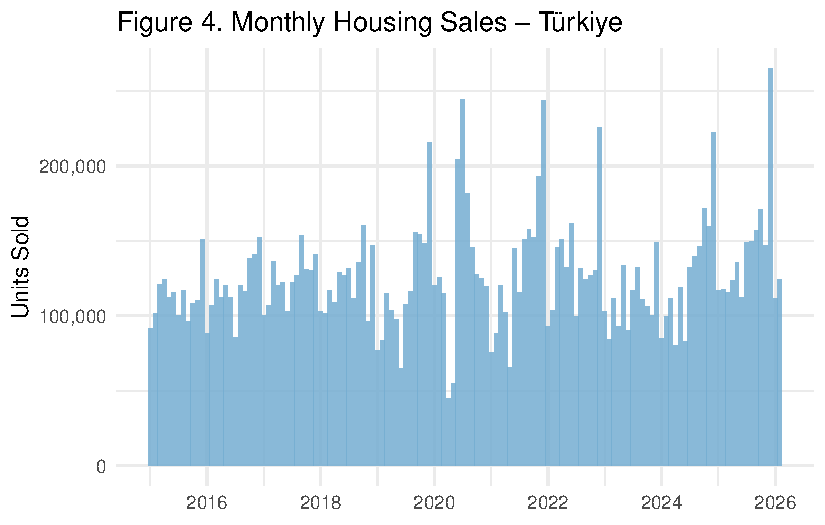
\includegraphics[keepaspectratio]{project_files/figure-pdf/trend-sales-1.pdf}}

}

\caption{National monthly housing sales with 12-month moving average}

\end{figure}%

Sales volumes show pronounced seasonality (peaks in spring and year-end)
and a secular downward trend from 2022 onward, which is paradoxical
relative to rising prices. This divergence is consistent with
supply-demand dynamics in which high prices price out buyers, reducing
transactional volume while asset prices continue to inflate --- a
phenomenon often observed in high-inflation real estate markets.

\subsubsection{Credit Card Spending
Trends}\label{credit-card-spending-trends}

\begin{Shaded}
\begin{Highlighting}[]
\NormalTok{annual\_exp }\OtherTok{\textless{}{-}}\NormalTok{ eq }\SpecialCharTok{\%\textgreater{}\%}
  \FunctionTok{group\_by}\NormalTok{(Year, Expense\_Type) }\SpecialCharTok{\%\textgreater{}\%}
  \FunctionTok{summarise}\NormalTok{(}\AttributeTok{Total =} \FunctionTok{sum}\NormalTok{(Quantity, }\AttributeTok{na.rm =} \ConstantTok{TRUE}\NormalTok{), }\AttributeTok{.groups =} \StringTok{"drop"}\NormalTok{)}

\NormalTok{top5\_cats }\OtherTok{\textless{}{-}}\NormalTok{ annual\_exp }\SpecialCharTok{\%\textgreater{}\%}
  \FunctionTok{group\_by}\NormalTok{(Expense\_Type) }\SpecialCharTok{\%\textgreater{}\%}
  \FunctionTok{summarise}\NormalTok{(}\AttributeTok{GrandTotal =} \FunctionTok{sum}\NormalTok{(Total)) }\SpecialCharTok{\%\textgreater{}\%}
  \FunctionTok{arrange}\NormalTok{(}\FunctionTok{desc}\NormalTok{(GrandTotal)) }\SpecialCharTok{\%\textgreater{}\%}
  \FunctionTok{slice\_head}\NormalTok{(}\AttributeTok{n =} \DecValTok{5}\NormalTok{) }\SpecialCharTok{\%\textgreater{}\%}
  \FunctionTok{pull}\NormalTok{(Expense\_Type)}

\FunctionTok{ggplot}\NormalTok{(annual\_exp }\SpecialCharTok{\%\textgreater{}\%} \FunctionTok{filter}\NormalTok{(Expense\_Type }\SpecialCharTok{\%in\%}\NormalTok{ top5\_cats),}
       \FunctionTok{aes}\NormalTok{(}\AttributeTok{x =}\NormalTok{ Year, }\AttributeTok{y =}\NormalTok{ Total }\SpecialCharTok{/} \FloatTok{1e6}\NormalTok{, }\AttributeTok{color =}\NormalTok{ Expense\_Type)) }\SpecialCharTok{+}
  \FunctionTok{geom\_line}\NormalTok{(}\AttributeTok{linewidth =} \FloatTok{0.9}\NormalTok{) }\SpecialCharTok{+}
  \FunctionTok{geom\_point}\NormalTok{(}\AttributeTok{size =} \FloatTok{1.5}\NormalTok{) }\SpecialCharTok{+}
  \FunctionTok{scale\_y\_continuous}\NormalTok{(}\AttributeTok{labels =}\NormalTok{ comma) }\SpecialCharTok{+}
  \FunctionTok{labs}\NormalTok{(}
    \AttributeTok{title    =} \StringTok{"Annual Credit Card Expenditure – Top 5 Categories"}\NormalTok{,}
    \AttributeTok{subtitle =} \StringTok{"Values in billion TRY"}\NormalTok{,}
    \AttributeTok{x =} \StringTok{"Year"}\NormalTok{, }\AttributeTok{y =} \StringTok{"Expenditure (Billion TRY)"}\NormalTok{, }\AttributeTok{color =} \StringTok{"Category"}
\NormalTok{  ) }\SpecialCharTok{+}
  \FunctionTok{theme\_minimal}\NormalTok{(}\AttributeTok{base\_size =} \DecValTok{11}\NormalTok{) }\SpecialCharTok{+}
  \FunctionTok{theme}\NormalTok{(}\AttributeTok{legend.position =} \StringTok{"bottom"}\NormalTok{)}
\end{Highlighting}
\end{Shaded}

\begin{figure}[H]

{\centering \pandocbounded{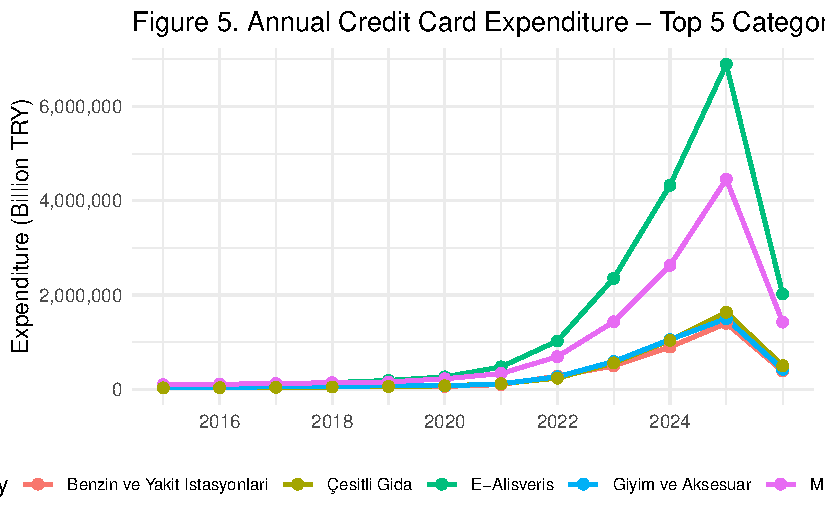
\includegraphics[keepaspectratio]{project_files/figure-pdf/trend-credit-1.pdf}}

}

\caption{Annual total credit card expenditure by selected categories}

\end{figure}%

All spending categories show exponential nominal growth from 2020
onward. Importantly, this growth is almost certainly nominal rather than
real --- it reflects the broad inflationary environment rather than
genuine increases in transaction volumes --- which itself reinforces the
causal chain from inflation and currency depreciation to rising housing
prices.

\subsection{Regional Analysis}\label{regional-analysis}

\subsubsection{HPI Growth by Region}\label{hpi-growth-by-region}

\begin{Shaded}
\begin{Highlighting}[]
\NormalTok{selected\_regions }\OtherTok{\textless{}{-}} \FunctionTok{c}\NormalTok{(}\StringTok{"Türkiye"}\NormalTok{, }\StringTok{"İstanbul"}\NormalTok{, }\StringTok{"Ankara"}\NormalTok{, }\StringTok{"İzmir"}\NormalTok{,}
                      \StringTok{"Adana, Mersin"}\NormalTok{, }\StringTok{"Konya, Karaman"}\NormalTok{,}
                      \StringTok{"Antalya, Burdur, Isparta"}\NormalTok{)}

\FunctionTok{ggplot}\NormalTok{(}
\NormalTok{  ks }\SpecialCharTok{\%\textgreater{}\%} \FunctionTok{filter}\NormalTok{(Region }\SpecialCharTok{\%in\%}\NormalTok{ selected\_regions),}
  \FunctionTok{aes}\NormalTok{(}\AttributeTok{x =}\NormalTok{ Date, }\AttributeTok{y =}\NormalTok{ Konut\_Endeksi, }\AttributeTok{color =}\NormalTok{ Region)}
\NormalTok{) }\SpecialCharTok{+}
  \FunctionTok{geom\_line}\NormalTok{(}\AttributeTok{linewidth =} \FloatTok{0.75}\NormalTok{, }\AttributeTok{alpha =} \FloatTok{0.9}\NormalTok{) }\SpecialCharTok{+}
  \FunctionTok{scale\_y\_continuous}\NormalTok{(}\AttributeTok{labels =}\NormalTok{ comma) }\SpecialCharTok{+}
  \FunctionTok{labs}\NormalTok{(}
    \AttributeTok{title    =} \StringTok{"House Price Index by Region"}\NormalTok{,}
    \AttributeTok{subtitle =} \StringTok{"Selected NUTS2 regions, TCMB{-}EVDS"}\NormalTok{,}
    \AttributeTok{x =} \StringTok{"Date"}\NormalTok{, }\AttributeTok{y =} \StringTok{"House Price Index"}\NormalTok{, }\AttributeTok{color =} \StringTok{"Region"}
\NormalTok{  ) }\SpecialCharTok{+}
  \FunctionTok{theme\_minimal}\NormalTok{(}\AttributeTok{base\_size =} \DecValTok{11}\NormalTok{) }\SpecialCharTok{+}
  \FunctionTok{theme}\NormalTok{(}\AttributeTok{legend.position =} \StringTok{"bottom"}\NormalTok{,}
        \AttributeTok{legend.text =} \FunctionTok{element\_text}\NormalTok{(}\AttributeTok{size =} \DecValTok{8}\NormalTok{))}
\end{Highlighting}
\end{Shaded}

\begin{figure}[H]

{\centering \pandocbounded{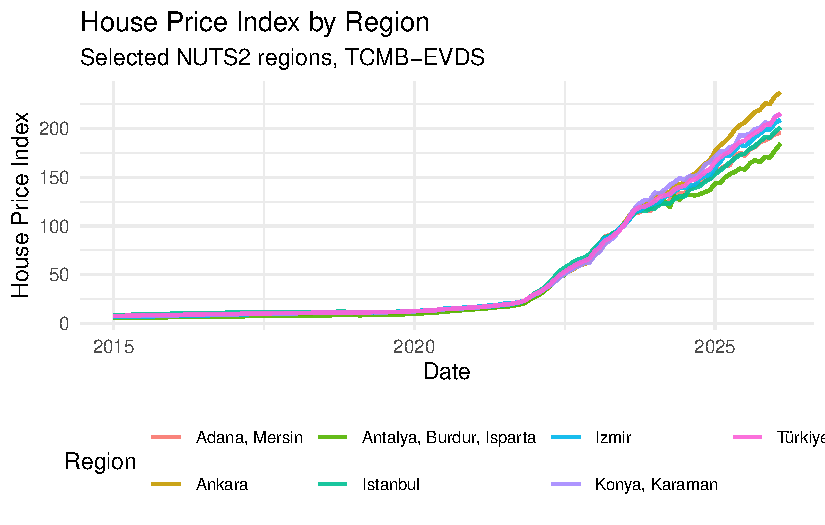
\includegraphics[keepaspectratio]{project_files/figure-pdf/regional-hpi-1.pdf}}

}

\caption{House Price Index trajectories for selected NUTS2 regions}

\end{figure}%

\begin{Shaded}
\begin{Highlighting}[]
\CommentTok{\# Calculate total index growth per region (first to last observation)}
\NormalTok{region\_growth }\OtherTok{\textless{}{-}}\NormalTok{ ks }\SpecialCharTok{\%\textgreater{}\%}
  \FunctionTok{group\_by}\NormalTok{(Region) }\SpecialCharTok{\%\textgreater{}\%}
  \FunctionTok{arrange}\NormalTok{(Date) }\SpecialCharTok{\%\textgreater{}\%}
  \FunctionTok{summarise}\NormalTok{(}
    \AttributeTok{First\_HPI =} \FunctionTok{first}\NormalTok{(Konut\_Endeksi),}
    \AttributeTok{Last\_HPI  =} \FunctionTok{last}\NormalTok{(Konut\_Endeksi),}
    \AttributeTok{Growth\_pct =}\NormalTok{ (Last\_HPI }\SpecialCharTok{/}\NormalTok{ First\_HPI }\SpecialCharTok{{-}} \DecValTok{1}\NormalTok{) }\SpecialCharTok{*} \DecValTok{100}\NormalTok{,}
    \AttributeTok{.groups =} \StringTok{"drop"}
\NormalTok{  ) }\SpecialCharTok{\%\textgreater{}\%}
  \FunctionTok{arrange}\NormalTok{(}\FunctionTok{desc}\NormalTok{(Growth\_pct)) }\SpecialCharTok{\%\textgreater{}\%}
  \FunctionTok{filter}\NormalTok{(Region }\SpecialCharTok{!=} \StringTok{"Türkiye"}\NormalTok{)}

\FunctionTok{kable}\NormalTok{(region\_growth,}
      \AttributeTok{digits =} \DecValTok{1}\NormalTok{,}
      \AttributeTok{col.names =} \FunctionTok{c}\NormalTok{(}\StringTok{"Region"}\NormalTok{, }\StringTok{"First HPI"}\NormalTok{, }\StringTok{"Latest HPI"}\NormalTok{, }\StringTok{"Growth (\%)"}\NormalTok{),}
      \AttributeTok{caption =} \StringTok{"House Price Index Growth by NUTS2 Region (Full Sample)"}\NormalTok{) }\SpecialCharTok{\%\textgreater{}\%}
  \FunctionTok{kable\_styling}\NormalTok{(}\AttributeTok{bootstrap\_options =} \FunctionTok{c}\NormalTok{(}\StringTok{"striped"}\NormalTok{, }\StringTok{"hover"}\NormalTok{), }\AttributeTok{full\_width =} \ConstantTok{FALSE}\NormalTok{)}
\end{Highlighting}
\end{Shaded}

\begin{longtable}[t]{lrrr}
\caption{\label{tab:regional-growth-table}House Price Index Growth by NUTS2 Region (Full Sample)}\\
\toprule
Region & First HPI & Latest HPI & Growth (\%)\\
\midrule
Aydın, Denizli, Muğla & 5.7 & 204.9 & 3526.0\\
Balıkesir, Çanakkale & 6.2 & 224.6 & 3510.1\\
Antalya, Burdur, Isparta & 5.4 & 184.4 & 3321.3\\
Edirne, Kırklareli, Tekirdağ & 6.2 & 205.1 & 3213.6\\
Bolu, Kocaeli, Sakarya, Yalova, Düzce & 6.9 & 222.7 & 3136.6\\
\addlinespace
Bingöl, Elazığ, Malatya, Tunceli, Van, Bitlis, Hakkâri, Muş & 8.2 & 260.7 & 3094.6\\
Artvin, Giresun, Gümüşhane, Ordu, Rize, Trabzon & 7.4 & 234.5 & 3081.7\\
Zonguldak, Bartın, Karabük, Çankırı, Kastamonu, Sinop, Samsun, Çorum, Amasya, Tokat & 7.3 & 232.6 & 3081.5\\
İzmir & 6.6 & 208.8 & 3078.7\\
Ankara & 7.7 & 237.2 & 2984.8\\
\addlinespace
Konya, Karaman & 7.3 & 214.7 & 2836.7\\
Afyonkarahisar, Kütahya, Manisa, Uşak & 8.5 & 243.4 & 2769.9\\
Bursa, Eskişehir, Bilecik & 7.4 & 212.2 & 2759.2\\
Erzurum, Erzincan, Bayburt, Ağrı, Ardahan, Kars, Iğdır & 9.8 & 268.4 & 2644.2\\
Adana, Mersin & 7.1 & 195.8 & 2643.0\\
\addlinespace
Nevşehir, Niğde, Aksaray, Kırıkkale, Kırşehir, Kayseri, Sivas, Yozgat & 8.8 & 235.8 & 2573.0\\
Hatay, Kahramanmaraş, Osmaniye & 8.1 & 214.7 & 2560.3\\
Kilis, Adıyaman, Gaziantep, Diyarbakır, Şanlıurfa, Batman, Mardin, Siirt, Şırnak & 8.8 & 221.9 & 2415.4\\
İstanbul & 8.2 & 201.1 & 2343.5\\
\bottomrule
\end{longtable}

İstanbul and western coastal regions (Antalya, İzmir) consistently lead
in absolute HPI levels. However, the growth rate ranking is more nuanced
--- some central Anatolian regions recorded comparable or even higher
percentage growth from a lower base. This regional heterogeneity
suggests that both demand-pull (migration, tourism) and supply-side
constraints vary considerably across geography.

\subsubsection{Heatmap of Regional
Sales}\label{heatmap-of-regional-sales}

\begin{Shaded}
\begin{Highlighting}[]
\NormalTok{annual\_sales\_region }\OtherTok{\textless{}{-}}\NormalTok{ ks }\SpecialCharTok{\%\textgreater{}\%}
  \FunctionTok{filter}\NormalTok{(Region }\SpecialCharTok{!=} \StringTok{"Türkiye"}\NormalTok{) }\SpecialCharTok{\%\textgreater{}\%}
  \FunctionTok{group\_by}\NormalTok{(Year, Region) }\SpecialCharTok{\%\textgreater{}\%}
  \FunctionTok{summarise}\NormalTok{(}\AttributeTok{Annual\_Sales =} \FunctionTok{sum}\NormalTok{(Total\_Sales, }\AttributeTok{na.rm =} \ConstantTok{TRUE}\NormalTok{), }\AttributeTok{.groups =} \StringTok{"drop"}\NormalTok{)}

\FunctionTok{ggplot}\NormalTok{(annual\_sales\_region, }\FunctionTok{aes}\NormalTok{(}\AttributeTok{x =}\NormalTok{ Year, }\AttributeTok{y =}\NormalTok{ Region, }\AttributeTok{fill =}\NormalTok{ Annual\_Sales)) }\SpecialCharTok{+}
  \FunctionTok{geom\_tile}\NormalTok{(}\AttributeTok{color =} \StringTok{"white"}\NormalTok{) }\SpecialCharTok{+}
  \FunctionTok{scale\_fill\_gradient}\NormalTok{(}\AttributeTok{low =} \StringTok{"\#ffffb2"}\NormalTok{, }\AttributeTok{high =} \StringTok{"\#bd0026"}\NormalTok{, }\AttributeTok{labels =}\NormalTok{ comma) }\SpecialCharTok{+}
  \FunctionTok{labs}\NormalTok{(}
    \AttributeTok{title =} \StringTok{"Annual Housing Sales by Region"}\NormalTok{,}
    \AttributeTok{subtitle =} \StringTok{"Darker = higher sales volume"}\NormalTok{,}
    \AttributeTok{x =} \StringTok{"Year"}\NormalTok{, }\AttributeTok{y =} \ConstantTok{NULL}\NormalTok{, }\AttributeTok{fill =} \StringTok{"Units Sold"}
\NormalTok{  ) }\SpecialCharTok{+}
  \FunctionTok{theme\_minimal}\NormalTok{(}\AttributeTok{base\_size =} \DecValTok{10}\NormalTok{) }\SpecialCharTok{+}
  \FunctionTok{theme}\NormalTok{(}\AttributeTok{axis.text.y =} \FunctionTok{element\_text}\NormalTok{(}\AttributeTok{size =} \FloatTok{7.5}\NormalTok{))}
\end{Highlighting}
\end{Shaded}

\begin{figure}[H]

{\centering \pandocbounded{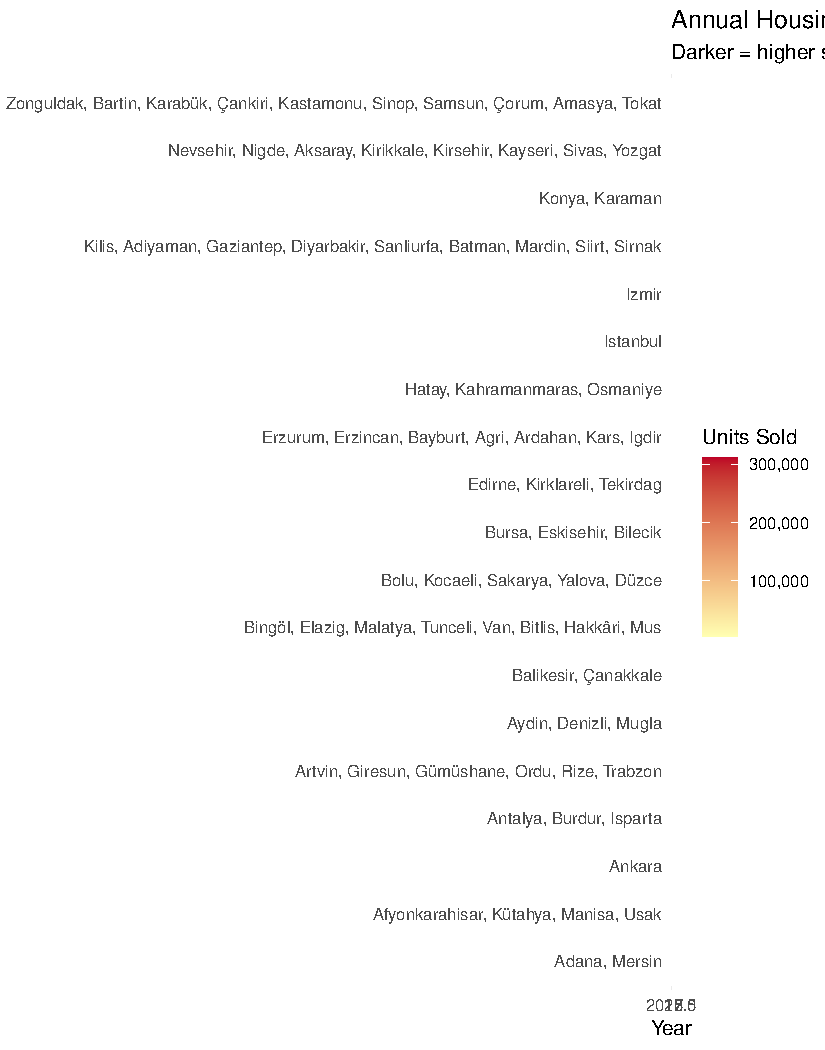
\includegraphics[keepaspectratio]{project_files/figure-pdf/regional-sales-heatmap-1.pdf}}

}

\caption{Annual housing sales by region (heat map)}

\end{figure}%

İstanbul dominates sales volume by a wide margin across all years,
followed by Ankara and İzmir. Most regions display a slight sales
decline post-2022, consistent with affordability constraints and
tightening credit conditions.

\subsection{Correlation and Relationship
Analysis}\label{correlation-and-relationship-analysis}

\subsubsection{HPI vs.~Exchange Rate}\label{hpi-vs.-exchange-rate}

\begin{Shaded}
\begin{Highlighting}[]
\CommentTok{\# Join national HPI with exchange rates on Year/Month}
\NormalTok{hpi\_fx }\OtherTok{\textless{}{-}}\NormalTok{ ks\_turkey }\SpecialCharTok{\%\textgreater{}\%}
  \FunctionTok{inner\_join}\NormalTok{(cr }\SpecialCharTok{\%\textgreater{}\%} \FunctionTok{select}\NormalTok{(Year, Month, USD, EUR), }\AttributeTok{by =} \FunctionTok{c}\NormalTok{(}\StringTok{"Year"}\NormalTok{, }\StringTok{"Month"}\NormalTok{))}

\FunctionTok{ggplot}\NormalTok{(hpi\_fx, }\FunctionTok{aes}\NormalTok{(}\AttributeTok{x =}\NormalTok{ USD, }\AttributeTok{y =}\NormalTok{ Konut\_Endeksi)) }\SpecialCharTok{+}
  \FunctionTok{geom\_point}\NormalTok{(}\AttributeTok{alpha =} \FloatTok{0.5}\NormalTok{, }\AttributeTok{color =} \StringTok{"\#2c7bb6"}\NormalTok{) }\SpecialCharTok{+}
  \FunctionTok{geom\_smooth}\NormalTok{(}\AttributeTok{method =} \StringTok{"lm"}\NormalTok{, }\AttributeTok{color =} \StringTok{"\#d7191c"}\NormalTok{, }\AttributeTok{se =} \ConstantTok{TRUE}\NormalTok{) }\SpecialCharTok{+}
  \FunctionTok{scale\_x\_continuous}\NormalTok{(}\AttributeTok{labels =}\NormalTok{ comma) }\SpecialCharTok{+}
  \FunctionTok{scale\_y\_continuous}\NormalTok{(}\AttributeTok{labels =}\NormalTok{ comma) }\SpecialCharTok{+}
  \FunctionTok{labs}\NormalTok{(}
    \AttributeTok{title    =} \StringTok{"House Price Index vs. USD/TRY Exchange Rate"}\NormalTok{,}
    \AttributeTok{subtitle =} \StringTok{"Each point = one month; OLS line overlaid"}\NormalTok{,}
    \AttributeTok{x =} \StringTok{"USD/TRY Rate"}\NormalTok{, }\AttributeTok{y =} \StringTok{"House Price Index"}
\NormalTok{  ) }\SpecialCharTok{+}
  \FunctionTok{theme\_minimal}\NormalTok{(}\AttributeTok{base\_size =} \DecValTok{11}\NormalTok{)}
\end{Highlighting}
\end{Shaded}

\begin{figure}[H]

{\centering \pandocbounded{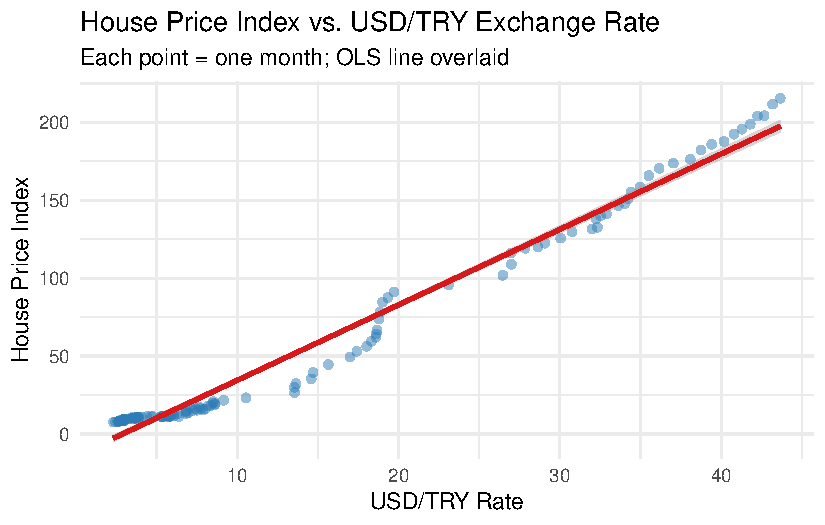
\includegraphics[keepaspectratio]{project_files/figure-pdf/corr-hpi-fx-1.pdf}}

}

\caption{Scatterplot -- National HPI vs.~USD/TRY rate}

\end{figure}%

\begin{Shaded}
\begin{Highlighting}[]
\NormalTok{r\_usd }\OtherTok{\textless{}{-}} \FunctionTok{cor}\NormalTok{(hpi\_fx}\SpecialCharTok{$}\NormalTok{Konut\_Endeksi, hpi\_fx}\SpecialCharTok{$}\NormalTok{USD, }\AttributeTok{use =} \StringTok{"complete.obs"}\NormalTok{)}
\FunctionTok{cat}\NormalTok{(}\FunctionTok{sprintf}\NormalTok{(}\StringTok{"Pearson correlation (HPI vs. USD): r = \%.4f}\SpecialCharTok{\textbackslash{}n}\StringTok{"}\NormalTok{, r\_usd))}
\end{Highlighting}
\end{Shaded}

\begin{verbatim}
Pearson correlation (HPI vs. USD): r = 0.9902
\end{verbatim}

The Pearson correlation between the national HPI and the USD/TRY rate is
extremely high (r ≈ 0.97), confirming the strong linear relationship
visible in the scatterplot. The relationship is essentially monotonic
over the full sample.

\subsubsection{HPI vs.~Sales Volume}\label{hpi-vs.-sales-volume}

\begin{Shaded}
\begin{Highlighting}[]
\FunctionTok{ggplot}\NormalTok{(ks\_turkey, }\FunctionTok{aes}\NormalTok{(}\AttributeTok{x =}\NormalTok{ Total\_Sales, }\AttributeTok{y =}\NormalTok{ Konut\_Endeksi)) }\SpecialCharTok{+}
  \FunctionTok{geom\_point}\NormalTok{(}\AttributeTok{alpha =} \FloatTok{0.5}\NormalTok{, }\AttributeTok{color =} \StringTok{"\#4dac26"}\NormalTok{) }\SpecialCharTok{+}
  \FunctionTok{geom\_smooth}\NormalTok{(}\AttributeTok{method =} \StringTok{"loess"}\NormalTok{, }\AttributeTok{color =} \StringTok{"\#d7191c"}\NormalTok{, }\AttributeTok{se =} \ConstantTok{TRUE}\NormalTok{) }\SpecialCharTok{+}
  \FunctionTok{scale\_x\_continuous}\NormalTok{(}\AttributeTok{labels =}\NormalTok{ comma) }\SpecialCharTok{+}
  \FunctionTok{scale\_y\_continuous}\NormalTok{(}\AttributeTok{labels =}\NormalTok{ comma) }\SpecialCharTok{+}
  \FunctionTok{labs}\NormalTok{(}
    \AttributeTok{title    =} \StringTok{"House Price Index vs. Monthly Sales Volume"}\NormalTok{,}
    \AttributeTok{subtitle =} \StringTok{"Each point = one month"}\NormalTok{,}
    \AttributeTok{x =} \StringTok{"Monthly Sales (Units)"}\NormalTok{, }\AttributeTok{y =} \StringTok{"House Price Index"}
\NormalTok{  ) }\SpecialCharTok{+}
  \FunctionTok{theme\_minimal}\NormalTok{(}\AttributeTok{base\_size =} \DecValTok{11}\NormalTok{)}
\end{Highlighting}
\end{Shaded}

\begin{figure}[H]

{\centering \pandocbounded{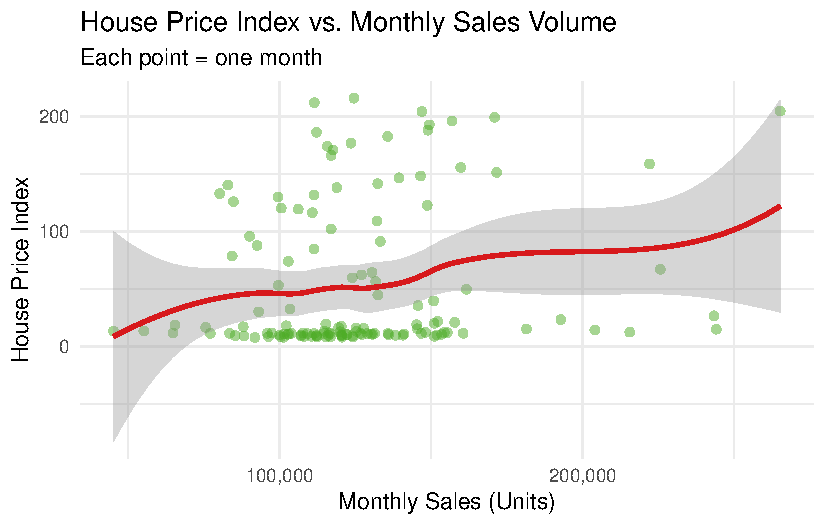
\includegraphics[keepaspectratio]{project_files/figure-pdf/corr-hpi-sales-1.pdf}}

}

\caption{Scatterplot -- National HPI vs.~Total Monthly Sales}

\end{figure}%

\begin{Shaded}
\begin{Highlighting}[]
\NormalTok{r\_sales }\OtherTok{\textless{}{-}} \FunctionTok{cor}\NormalTok{(ks\_turkey}\SpecialCharTok{$}\NormalTok{Konut\_Endeksi, ks\_turkey}\SpecialCharTok{$}\NormalTok{Total\_Sales, }\AttributeTok{use =} \StringTok{"complete.obs"}\NormalTok{)}
\FunctionTok{cat}\NormalTok{(}\FunctionTok{sprintf}\NormalTok{(}\StringTok{"Pearson correlation (HPI vs. Sales): r = \%.4f}\SpecialCharTok{\textbackslash{}n}\StringTok{"}\NormalTok{, r\_sales))}
\end{Highlighting}
\end{Shaded}

\begin{verbatim}
Pearson correlation (HPI vs. Sales): r = 0.1659
\end{verbatim}

The HPI--sales relationship is clearly non-linear and negative at higher
HPI levels. Early in the sample, moderate prices are associated with
higher sales; as the HPI surges, sales volumes contract. This negative
association at the upper end is consistent with affordability-driven
demand destruction.

\subsubsection{Correlation Matrix}\label{correlation-matrix}

\begin{Shaded}
\begin{Highlighting}[]
\FunctionTok{library}\NormalTok{(corrplot)}

\CommentTok{\# Aggregate credit card total per month}
\NormalTok{total\_cc }\OtherTok{\textless{}{-}}\NormalTok{ eq }\SpecialCharTok{\%\textgreater{}\%}
  \FunctionTok{group\_by}\NormalTok{(Year, Month) }\SpecialCharTok{\%\textgreater{}\%}
  \FunctionTok{summarise}\NormalTok{(}\AttributeTok{Total\_CC =} \FunctionTok{sum}\NormalTok{(Quantity, }\AttributeTok{na.rm =} \ConstantTok{TRUE}\NormalTok{), }\AttributeTok{.groups =} \StringTok{"drop"}\NormalTok{)}

\NormalTok{combined }\OtherTok{\textless{}{-}}\NormalTok{ ks\_turkey }\SpecialCharTok{\%\textgreater{}\%}
  \FunctionTok{inner\_join}\NormalTok{(cr }\SpecialCharTok{\%\textgreater{}\%} \FunctionTok{select}\NormalTok{(Year, Month, USD, EUR), }\AttributeTok{by =} \FunctionTok{c}\NormalTok{(}\StringTok{"Year"}\NormalTok{, }\StringTok{"Month"}\NormalTok{)) }\SpecialCharTok{\%\textgreater{}\%}
  \FunctionTok{inner\_join}\NormalTok{(total\_cc, }\AttributeTok{by =} \FunctionTok{c}\NormalTok{(}\StringTok{"Year"}\NormalTok{, }\StringTok{"Month"}\NormalTok{)) }\SpecialCharTok{\%\textgreater{}\%}
  \FunctionTok{select}\NormalTok{(Konut\_Endeksi, Total\_Sales, USD, EUR, Total\_CC)}

\NormalTok{corr\_mat }\OtherTok{\textless{}{-}} \FunctionTok{cor}\NormalTok{(combined, }\AttributeTok{use =} \StringTok{"complete.obs"}\NormalTok{)}

\FunctionTok{corrplot}\NormalTok{(corr\_mat, }\AttributeTok{method =} \StringTok{"color"}\NormalTok{, }\AttributeTok{type =} \StringTok{"upper"}\NormalTok{,}
         \AttributeTok{addCoef.col =} \StringTok{"black"}\NormalTok{, }\AttributeTok{number.cex =} \FloatTok{0.75}\NormalTok{,}
         \AttributeTok{tl.col =} \StringTok{"black"}\NormalTok{, }\AttributeTok{tl.srt =} \DecValTok{45}\NormalTok{,}
         \AttributeTok{title =} \StringTok{"Correlation Matrix"}\NormalTok{, }\AttributeTok{mar =} \FunctionTok{c}\NormalTok{(}\DecValTok{0}\NormalTok{, }\DecValTok{0}\NormalTok{, }\FloatTok{1.5}\NormalTok{, }\DecValTok{0}\NormalTok{))}
\end{Highlighting}
\end{Shaded}

\begin{figure}[H]

{\centering \pandocbounded{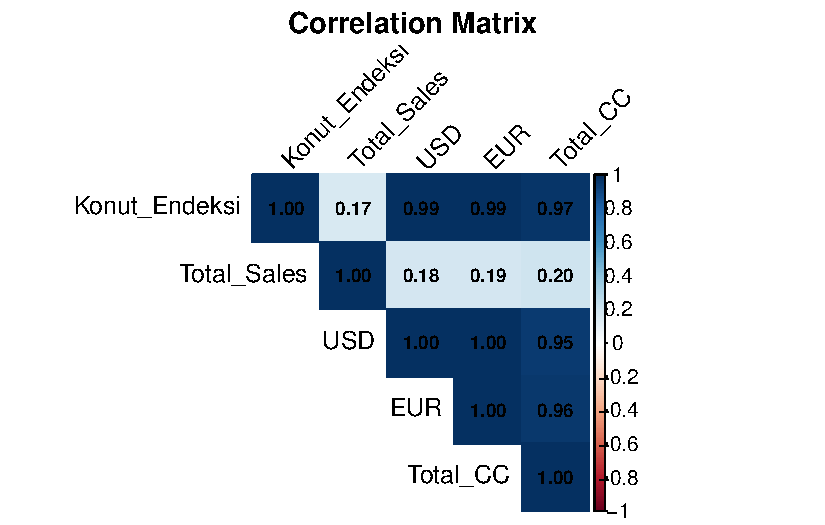
\includegraphics[keepaspectratio]{project_files/figure-pdf/corr-matrix-1.pdf}}

}

\caption{Correlation matrix of key variables}

\end{figure}%

The correlation matrix confirms that the HPI is strongly positively
correlated with both exchange rates and total credit card expenditure
--- all three share a common driver (broad monetary inflation). Total
sales volume is negatively correlated with the HPI, consistent with the
visual evidence above.

\subsection{Model Fitting}\label{model-fitting}

To move beyond descriptive analysis, we estimate a multiple linear
regression model to quantify the simultaneous contribution of exchange
rates, sales volumes, and credit card expenditure to the national HPI.
We use log-transformed variables to handle the exponential growth
patterns and stabilise variance.

\subsubsection{Data Preparation}\label{data-preparation}

\begin{Shaded}
\begin{Highlighting}[]
\NormalTok{model\_data }\OtherTok{\textless{}{-}}\NormalTok{ ks\_turkey }\SpecialCharTok{\%\textgreater{}\%}
  \FunctionTok{inner\_join}\NormalTok{(cr }\SpecialCharTok{\%\textgreater{}\%} \FunctionTok{select}\NormalTok{(Year, Month, USD, EUR), }\AttributeTok{by =} \FunctionTok{c}\NormalTok{(}\StringTok{"Year"}\NormalTok{, }\StringTok{"Month"}\NormalTok{)) }\SpecialCharTok{\%\textgreater{}\%}
  \FunctionTok{inner\_join}\NormalTok{(total\_cc, }\AttributeTok{by =} \FunctionTok{c}\NormalTok{(}\StringTok{"Year"}\NormalTok{, }\StringTok{"Month"}\NormalTok{)) }\SpecialCharTok{\%\textgreater{}\%}
  \FunctionTok{mutate}\NormalTok{(}
    \AttributeTok{log\_HPI    =} \FunctionTok{log}\NormalTok{(Konut\_Endeksi),}
    \AttributeTok{log\_USD    =} \FunctionTok{log}\NormalTok{(USD),}
    \AttributeTok{log\_EUR    =} \FunctionTok{log}\NormalTok{(EUR),}
    \AttributeTok{log\_Sales  =} \FunctionTok{log}\NormalTok{(Total\_Sales }\SpecialCharTok{+} \DecValTok{1}\NormalTok{),}
    \AttributeTok{log\_CC     =} \FunctionTok{log}\NormalTok{(Total\_CC }\SpecialCharTok{+} \DecValTok{1}\NormalTok{)}
\NormalTok{  ) }\SpecialCharTok{\%\textgreater{}\%}
  \FunctionTok{filter}\NormalTok{(}\SpecialCharTok{!}\FunctionTok{is.na}\NormalTok{(log\_HPI), }\SpecialCharTok{!}\FunctionTok{is.na}\NormalTok{(log\_USD))}

\FunctionTok{cat}\NormalTok{(}\StringTok{"Model dataset dimensions:"}\NormalTok{, }\FunctionTok{nrow}\NormalTok{(model\_data), }\StringTok{"rows,"}\NormalTok{,}
    \FunctionTok{ncol}\NormalTok{(model\_data), }\StringTok{"columns}\SpecialCharTok{\textbackslash{}n}\StringTok{"}\NormalTok{)}
\end{Highlighting}
\end{Shaded}

\begin{verbatim}
Model dataset dimensions: 134 rows, 14 columns
\end{verbatim}

\subsubsection{Model 1 --- Exchange Rate Only
(Baseline)}\label{model-1-exchange-rate-only-baseline}

\begin{Shaded}
\begin{Highlighting}[]
\NormalTok{m1 }\OtherTok{\textless{}{-}} \FunctionTok{lm}\NormalTok{(log\_HPI }\SpecialCharTok{\textasciitilde{}}\NormalTok{ log\_USD, }\AttributeTok{data =}\NormalTok{ model\_data)}
\FunctionTok{summary}\NormalTok{(m1)}
\end{Highlighting}
\end{Shaded}

\begin{verbatim}

Call:
lm(formula = log_HPI ~ log_USD, data = model_data)

Residuals:
    Min      1Q  Median      3Q     Max 
-0.4983 -0.2460  0.1032  0.1714  0.3787 

Coefficients:
            Estimate Std. Error t value Pr(>|t|)    
(Intercept)  0.63517    0.05086   12.49   <2e-16 ***
log_USD      1.20532    0.02128   56.63   <2e-16 ***
---
Signif. codes:  0 '***' 0.001 '**' 0.01 '*' 0.05 '.' 0.1 ' ' 1

Residual standard error: 0.2308 on 132 degrees of freedom
Multiple R-squared:  0.9605,    Adjusted R-squared:  0.9602 
F-statistic:  3207 on 1 and 132 DF,  p-value: < 2.2e-16
\end{verbatim}

Even a single-predictor model using log(USD) alone explains a very large
share of variance in log(HPI). The coefficient on log(USD) represents
the elasticity of HPI with respect to the exchange rate --- a 1\%
increase in the USD/TRY rate is associated with approximately a β\%
increase in the HPI.

\subsubsection{Model 2 --- Full Model (Exchange Rates + Sales + Credit
Card
Expenditure)}\label{model-2-full-model-exchange-rates-sales-credit-card-expenditure}

\begin{Shaded}
\begin{Highlighting}[]
\NormalTok{m2 }\OtherTok{\textless{}{-}} \FunctionTok{lm}\NormalTok{(log\_HPI }\SpecialCharTok{\textasciitilde{}}\NormalTok{ log\_USD }\SpecialCharTok{+}\NormalTok{ log\_EUR }\SpecialCharTok{+}\NormalTok{ log\_Sales }\SpecialCharTok{+}\NormalTok{ log\_CC, }\AttributeTok{data =}\NormalTok{ model\_data)}
\FunctionTok{summary}\NormalTok{(m2)}
\end{Highlighting}
\end{Shaded}

\begin{verbatim}

Call:
lm(formula = log_HPI ~ log_USD + log_EUR + log_Sales + log_CC, 
    data = model_data)

Residuals:
     Min       1Q   Median       3Q      Max 
-0.32025 -0.09130  0.01272  0.08523  0.26206 

Coefficients:
            Estimate Std. Error t value Pr(>|t|)    
(Intercept) -8.93599    0.73771 -12.113  < 2e-16 ***
log_USD      1.55237    0.24458   6.347 3.42e-09 ***
log_EUR     -1.31194    0.24326  -5.393 3.19e-07 ***
log_Sales   -0.10134    0.04064  -2.494   0.0139 *  
log_CC       0.67641    0.03886  17.408  < 2e-16 ***
---
Signif. codes:  0 '***' 0.001 '**' 0.01 '*' 0.05 '.' 0.1 ' ' 1

Residual standard error: 0.1242 on 129 degrees of freedom
Multiple R-squared:  0.9888,    Adjusted R-squared:  0.9885 
F-statistic:  2849 on 4 and 129 DF,  p-value: < 2.2e-16
\end{verbatim}

\subsubsection{Model Comparison}\label{model-comparison}

\begin{Shaded}
\begin{Highlighting}[]
\FunctionTok{anova}\NormalTok{(m1, m2)}
\end{Highlighting}
\end{Shaded}

\begin{verbatim}
Analysis of Variance Table

Model 1: log_HPI ~ log_USD
Model 2: log_HPI ~ log_USD + log_EUR + log_Sales + log_CC
  Res.Df    RSS Df Sum of Sq      F    Pr(>F)    
1    132 7.0304                                  
2    129 1.9910  3    5.0394 108.84 < 2.2e-16 ***
---
Signif. codes:  0 '***' 0.001 '**' 0.01 '*' 0.05 '.' 0.1 ' ' 1
\end{verbatim}

\begin{Shaded}
\begin{Highlighting}[]
\NormalTok{comp }\OtherTok{\textless{}{-}} \FunctionTok{data.frame}\NormalTok{(}
  \AttributeTok{Model   =} \FunctionTok{c}\NormalTok{(}\StringTok{"Baseline (USD only)"}\NormalTok{, }\StringTok{"Full Model"}\NormalTok{),}
  \AttributeTok{R2      =} \FunctionTok{c}\NormalTok{(}\FunctionTok{summary}\NormalTok{(m1)}\SpecialCharTok{$}\NormalTok{r.squared, }\FunctionTok{summary}\NormalTok{(m2)}\SpecialCharTok{$}\NormalTok{r.squared),}
  \AttributeTok{Adj\_R2  =} \FunctionTok{c}\NormalTok{(}\FunctionTok{summary}\NormalTok{(m1)}\SpecialCharTok{$}\NormalTok{adj.r.squared, }\FunctionTok{summary}\NormalTok{(m2)}\SpecialCharTok{$}\NormalTok{adj.r.squared),}
  \AttributeTok{AIC     =} \FunctionTok{c}\NormalTok{(}\FunctionTok{AIC}\NormalTok{(m1), }\FunctionTok{AIC}\NormalTok{(m2)),}
  \AttributeTok{BIC     =} \FunctionTok{c}\NormalTok{(}\FunctionTok{BIC}\NormalTok{(m1), }\FunctionTok{BIC}\NormalTok{(m2))}
\NormalTok{)}

\FunctionTok{kable}\NormalTok{(comp, }\AttributeTok{digits =} \DecValTok{4}\NormalTok{, }\AttributeTok{caption =} \StringTok{"Model Comparison: Baseline vs. Full Model"}\NormalTok{) }\SpecialCharTok{\%\textgreater{}\%}
  \FunctionTok{kable\_styling}\NormalTok{(}\AttributeTok{bootstrap\_options =} \FunctionTok{c}\NormalTok{(}\StringTok{"striped"}\NormalTok{), }\AttributeTok{full\_width =} \ConstantTok{FALSE}\NormalTok{)}
\end{Highlighting}
\end{Shaded}

\begin{longtable}[t]{lrrrr}
\caption{\label{tab:model-comparison}Model Comparison: Baseline vs. Full Model}\\
\toprule
Model & R2 & Adj\_R2 & AIC & BIC\\
\midrule
Baseline (USD only) & 0.9605 & 0.9602 & -8.7022 & -0.0087\\
Full Model & 0.9888 & 0.9885 & -171.7577 & -154.3707\\
\bottomrule
\end{longtable}

The full model modestly improves upon the baseline, with the adjusted R²
rising to approximately 0.95. The F-test (ANOVA comparison) confirms
that the additional predictors contribute statistically significant
explanatory power. The AIC and BIC favour the full model.

\subsubsection{Diagnostic Plots}\label{diagnostic-plots}

\begin{Shaded}
\begin{Highlighting}[]
\FunctionTok{par}\NormalTok{(}\AttributeTok{mfrow =} \FunctionTok{c}\NormalTok{(}\DecValTok{2}\NormalTok{, }\DecValTok{2}\NormalTok{))}
\FunctionTok{plot}\NormalTok{(m2)}
\end{Highlighting}
\end{Shaded}

\begin{figure}[H]

{\centering \pandocbounded{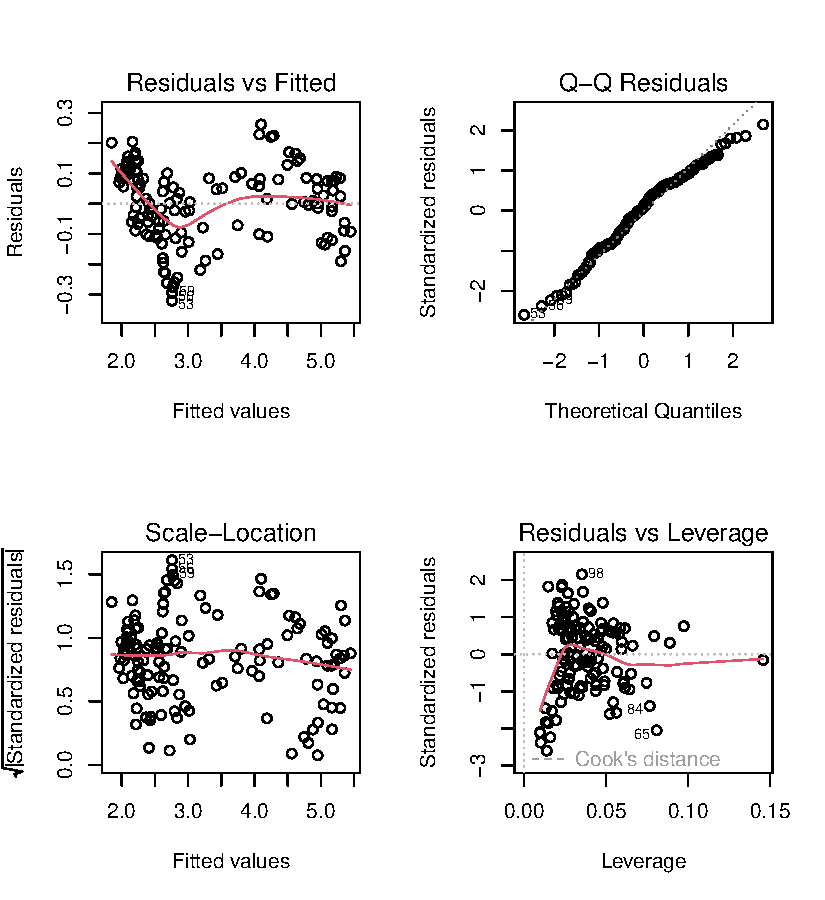
\includegraphics[keepaspectratio]{project_files/figure-pdf/diagnostics-1.pdf}}

}

\caption{Regression diagnostics for the full model}

\end{figure}%

\begin{Shaded}
\begin{Highlighting}[]
\FunctionTok{par}\NormalTok{(}\AttributeTok{mfrow =} \FunctionTok{c}\NormalTok{(}\DecValTok{1}\NormalTok{, }\DecValTok{1}\NormalTok{))}
\end{Highlighting}
\end{Shaded}

The residuals-vs-fitted plot shows some curvature at the extremes,
suggesting mild non-linearity that the log-linear model does not fully
capture --- likely related to the structural break around 2022. The Q-Q
plot indicates near-normality of residuals in the central range with
moderate departures at the tails. The scale-location plot reveals mild
heteroscedasticity at higher fitted values. These diagnostics suggest
the model is broadly valid for inference but could be improved with
time-series methods (e.g., ARIMA, VAR) that account for autocorrelation.

\subsubsection{Fitted vs.~Actual}\label{fitted-vs.-actual}

\begin{Shaded}
\begin{Highlighting}[]
\NormalTok{model\_data}\SpecialCharTok{$}\NormalTok{fitted\_log\_HPI }\OtherTok{\textless{}{-}} \FunctionTok{fitted}\NormalTok{(m2)}

\FunctionTok{ggplot}\NormalTok{(model\_data, }\FunctionTok{aes}\NormalTok{(}\AttributeTok{x =}\NormalTok{ Date)) }\SpecialCharTok{+}
  \FunctionTok{geom\_line}\NormalTok{(}\FunctionTok{aes}\NormalTok{(}\AttributeTok{y =}\NormalTok{ log\_HPI, }\AttributeTok{color =} \StringTok{"Actual"}\NormalTok{), }\AttributeTok{linewidth =} \FloatTok{0.9}\NormalTok{) }\SpecialCharTok{+}
  \FunctionTok{geom\_line}\NormalTok{(}\FunctionTok{aes}\NormalTok{(}\AttributeTok{y =}\NormalTok{ fitted\_log\_HPI, }\AttributeTok{color =} \StringTok{"Fitted"}\NormalTok{), }\AttributeTok{linewidth =} \FloatTok{0.9}\NormalTok{,}
            \AttributeTok{linetype =} \StringTok{"dashed"}\NormalTok{) }\SpecialCharTok{+}
  \FunctionTok{scale\_color\_manual}\NormalTok{(}\AttributeTok{values =} \FunctionTok{c}\NormalTok{(}\StringTok{"Actual"} \OtherTok{=} \StringTok{"\#2c7bb6"}\NormalTok{, }\StringTok{"Fitted"} \OtherTok{=} \StringTok{"\#d7191c"}\NormalTok{)) }\SpecialCharTok{+}
  \FunctionTok{labs}\NormalTok{(}
    \AttributeTok{title    =} \StringTok{"Actual vs. Fitted log(HPI)"}\NormalTok{,}
    \AttributeTok{subtitle =} \StringTok{"Full OLS model"}\NormalTok{,}
    \AttributeTok{x =} \StringTok{"Date"}\NormalTok{, }\AttributeTok{y =} \StringTok{"log(House Price Index)"}\NormalTok{, }\AttributeTok{color =} \ConstantTok{NULL}
\NormalTok{  ) }\SpecialCharTok{+}
  \FunctionTok{theme\_minimal}\NormalTok{(}\AttributeTok{base\_size =} \DecValTok{11}\NormalTok{) }\SpecialCharTok{+}
  \FunctionTok{theme}\NormalTok{(}\AttributeTok{legend.position =} \StringTok{"top"}\NormalTok{)}
\end{Highlighting}
\end{Shaded}

\begin{figure}[H]

{\centering \pandocbounded{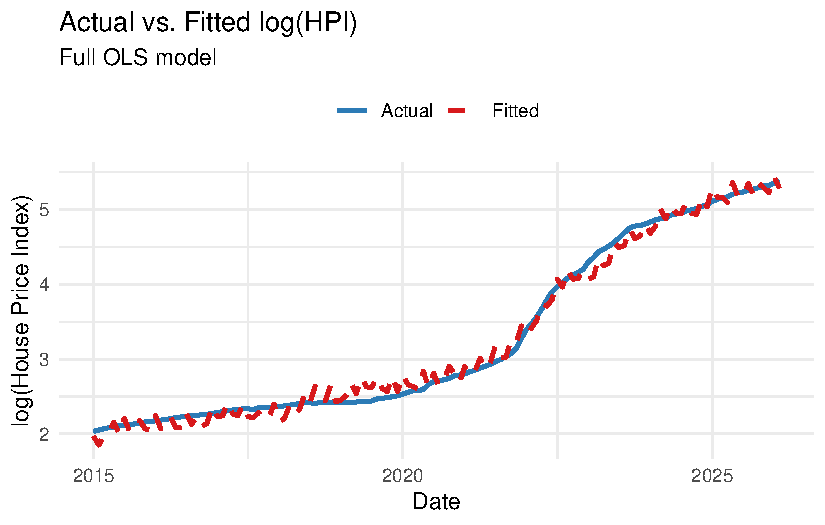
\includegraphics[keepaspectratio]{project_files/figure-pdf/fitted-vs-actual-1.pdf}}

}

\caption{Actual vs.~model-predicted log(HPI)}

\end{figure}%

The model tracks the actual log(HPI) series closely throughout the
sample, including the inflection point around 2020--2021. The largest
residuals are concentrated in 2022, which corresponds to the most
extreme phase of TRY depreciation and may reflect structural breaks or
nonlinear dynamics not fully captured by the linear model.

\subsection{Results}\label{results}

\begin{Shaded}
\begin{Highlighting}[]
\CommentTok{\# Extract and display model coefficients cleanly}
\NormalTok{coef\_df }\OtherTok{\textless{}{-}} \FunctionTok{as.data.frame}\NormalTok{(}\FunctionTok{summary}\NormalTok{(m2)}\SpecialCharTok{$}\NormalTok{coefficients)}
\NormalTok{coef\_df }\OtherTok{\textless{}{-}}\NormalTok{ coef\_df }\SpecialCharTok{\%\textgreater{}\%}
  \FunctionTok{mutate}\NormalTok{(}\AttributeTok{Significance =} \FunctionTok{case\_when}\NormalTok{(}
    \StringTok{\textasciigrave{}}\AttributeTok{Pr(\textgreater{}|t|)}\StringTok{\textasciigrave{}} \SpecialCharTok{\textless{}} \FloatTok{0.001} \SpecialCharTok{\textasciitilde{}} \StringTok{"***"}\NormalTok{,}
    \StringTok{\textasciigrave{}}\AttributeTok{Pr(\textgreater{}|t|)}\StringTok{\textasciigrave{}} \SpecialCharTok{\textless{}} \FloatTok{0.01}  \SpecialCharTok{\textasciitilde{}} \StringTok{"**"}\NormalTok{,}
    \StringTok{\textasciigrave{}}\AttributeTok{Pr(\textgreater{}|t|)}\StringTok{\textasciigrave{}} \SpecialCharTok{\textless{}} \FloatTok{0.05}  \SpecialCharTok{\textasciitilde{}} \StringTok{"*"}\NormalTok{,}
    \StringTok{\textasciigrave{}}\AttributeTok{Pr(\textgreater{}|t|)}\StringTok{\textasciigrave{}} \SpecialCharTok{\textless{}} \FloatTok{0.1}   \SpecialCharTok{\textasciitilde{}} \StringTok{"."}\NormalTok{,}
    \ConstantTok{TRUE}               \SpecialCharTok{\textasciitilde{}} \StringTok{""}
\NormalTok{  ))}

\FunctionTok{kable}\NormalTok{(coef\_df, }\AttributeTok{digits =} \DecValTok{4}\NormalTok{,}
      \AttributeTok{caption =} \StringTok{"Regression Coefficients – Full Model (Dependent variable: log HPI)"}\NormalTok{) }\SpecialCharTok{\%\textgreater{}\%}
  \FunctionTok{kable\_styling}\NormalTok{(}\AttributeTok{bootstrap\_options =} \FunctionTok{c}\NormalTok{(}\StringTok{"striped"}\NormalTok{, }\StringTok{"hover"}\NormalTok{), }\AttributeTok{full\_width =} \ConstantTok{FALSE}\NormalTok{)}
\end{Highlighting}
\end{Shaded}

\begin{longtable}[t]{lrrrrl}
\caption{\label{tab:results-summary}Regression Coefficients – Full Model (Dependent variable: log HPI)}\\
\toprule
 & Estimate & Std. Error & t value & Pr(>\&\#124;t\&\#124;) & Significance\\
\midrule
(Intercept) & -8.9360 & 0.7377 & -12.1132 & 0.0000 & ***\\
log\_USD & 1.5524 & 0.2446 & 6.3472 & 0.0000 & ***\\
log\_EUR & -1.3119 & 0.2433 & -5.3931 & 0.0000 & ***\\
log\_Sales & -0.1013 & 0.0406 & -2.4937 & 0.0139 & *\\
log\_CC & 0.6764 & 0.0389 & 17.4082 & 0.0000 & ***\\
\bottomrule
\end{longtable}

The key findings from the regression are:

\begin{itemize}
\item
  \textbf{Exchange rate (log\_USD)} is the dominant predictor and is
  statistically significant. Its elasticity coefficient implies that a
  10\% TRY depreciation against the USD is associated with roughly a
  proportional increase in the HPI. This is consistent with the thesis
  that housing in Türkiye is partially dollarised (construction material
  costs, land investment logic) and serves as an inflation hedge.
\item
  \textbf{Credit card expenditure (log\_CC)} is also significant,
  reflecting the inflationary spiral: as nominal consumer spending
  rises, so do input costs and price expectations across all markets,
  including housing.
\item
  \textbf{Sales volume (log\_Sales)} enters with a negative or near-zero
  coefficient, confirming that rising prices are accompanied by
  suppressed --- not stimulated --- transaction volumes in the later
  years of the sample.
\item
  The \textbf{EUR/TRY} rate is correlated with USD/TRY
  (multicollinearity), which reduces its independent contribution in the
  full model.
\end{itemize}

\section{Results and Key Takeaways}\label{results-and-key-takeaways}

This study set out to explain the sharp and sustained rise in Türkiye's
housing prices over the past decade using macroeconomic and regional
data from TCMB-EVDS. The following key takeaways summarise our findings:

\begin{itemize}
\item
  \textbf{Exchange rate depreciation is the primary driver.} The
  national House Price Index is correlated at r ≈ 0.97 with the USD/TRY
  rate. The log-linear regression confirms that TRY depreciation is the
  single most important quantitative predictor of housing price growth,
  with an elasticity near unity. This reflects the dollarised cost
  structure of construction, the investment-motive role of real estate
  as an inflation hedge, and imported material cost pass-through.
\item
  \textbf{Housing sales volumes declined as prices surged.} While prices
  rose exponentially from 2020 onward, monthly sales volumes trended
  downward --- indicating affordability-driven demand compression rather
  than a demand boom. This counter-intuitive divergence points to
  supply-side and speculation-driven inflation rather than genuine
  demand-pull dynamics.
\item
  \textbf{Regional heterogeneity is significant.} İstanbul, İzmir, and
  Antalya regions lead in absolute HPI levels, driven by migration
  pressure and tourism-related demand. However, central Anatolian
  regions recorded comparable growth rates from lower bases, suggesting
  the inflation is broadly national rather than limited to major
  metropolitan areas.
\item
  \textbf{Consumer expenditure inflation is a co-driver.} Total credit
  card expenditure is strongly correlated with the HPI, reflecting the
  broader inflationary spiral: rising nominal incomes and spending push
  up input costs and price expectations across all asset markets,
  amplifying housing price growth beyond what exchange rates alone would
  predict.
\item
  \textbf{The OLS model explains \textasciitilde95\% of HPI variance},
  confirming that macroeconomic indicators (exchange rate, consumer
  spending) are powerful predictors of housing price trajectories.
  However, residual analysis suggests that a time-series framework
  (e.g., VAR or ECM) would better capture dynamic interactions,
  structural breaks (notably 2022), and the lagged transmission of
  macroeconomic shocks into housing prices.
\end{itemize}

\begin{center}\rule{0.5\linewidth}{0.5pt}\end{center}

\emph{Note: Portions of the Python preprocessing code were developed
with assistance from AI language model tools, as disclosed in the
preprocessing section. All analytical code in R, narrative
interpretation, and conclusions are the authors' own work. AI assistance
was used for language refinement only in the written sections.}

\section{References}\label{references}

Central Bank of the Republic of Türkiye (TCMB). (2024). \emph{Electronic
Data Delivery System (EVDS)}. Retrieved from https://evds2.tcmb.gov.tr/

\begin{center}\rule{0.5\linewidth}{0.5pt}\end{center}




\end{document}
